\documentclass[12 pt]{article}
\usepackage[utf8]{inputenc}
\usepackage{graphicx}
\usepackage{amsmath}
\usepackage{amssymb}
\usepackage{multirow}
\usepackage{caption}
\usepackage{float}
\usepackage{subcaption}
\usepackage{hyperref}
\usepackage{pgf}
\usepackage{pgfpages}
\usepackage{textcomp}
\usepackage{lscape}
\usepackage{geometry}
\usepackage{pdflscape} 
\usepackage{placeins}
\usepackage{url}
\usepackage{natbib}
\usepackage[paper=A4]{typearea}
\graphicspath{ {figures/} }
\usepackage{array}
\usepackage{placeins}
\usepackage{afterpage}
\usepackage{bookmark}% faster updated bookmarks
\usepackage{xcolor}
%\usepackage{cite}
%\usepackage[a4paper,margin=1in]{geometry}



\pgfpagesdeclarelayout{boxed}
{
  \edef\pgfpageoptionborder{0pt}
}
{
  \pgfpagesphysicalpageoptions
  {%
    logical pages=1,%
  }
  \pgfpageslogicalpageoptions{1}
  {
    border code=\pgfsetlinewidth{2pt}\pgfstroke,%
    border shrink=\pgfpageoptionborder,%
    resized width=.95\pgfphysicalwidth,%
    resized height=.95\pgfphysicalheight,%
    center=\pgfpoint{.5\pgfphysicalwidth}{.5\pgfphysicalheight}%
  }%
}

\pgfpagesuselayout{boxed}

\title{Assignment 1}
\author{Abhijeet Mangela}
\date{November 2022}

\title{Assignment 1}
\author{Abhijeet Mangela}
\date{\today}

\begin{document}
\begin{titlepage}
\begin{center}

\textbf{\huge Design project report Group 7 \\ \vspace{0.5 cm} Week 5} \\

\vspace{2 cm}

\centering

\includegraphics[width=0.4\textwidth]{IIT_Madras_Logo.svg.png}
\label{fig:my_label}

\vspace{2 cm}

\Large{Abhijeet Mangela AE21B040 \\ \vspace{0.2 cm} Navin Yadav AE23M803 \\ \vspace{0.2 cm} Balamurugan S AE23M009 \\ \vspace{0.2 cm} Samarth R Krishna AE23M032 \\ \vspace{0.2 cm} Senthil B AE23M035 \\ \vspace{0.2 cm} Rajendran Anandhu Nair AE23M027 }

\vspace{1.0 cm}

\textbf{\Large Department of Aerospace Engineering } \\ \vspace{0.2 cm}
\textbf{\Large IIT Madras} \\ \vspace{0.2 cm}
\textbf{\Large India} \\ 

\normalsize

\end{center}
\end{titlepage}

\newpage
\vspace*{\fill}

%\begin{midpage}
\begin{center}
    \textbf{Abstract} \\ \vspace{0.5 cm}
\end{center}
Air quality is an essential measure of the quality of life of any living being. A decrease in air quality is easily linked with a reduction in the life expectancy of various plants and animals.
As a result, we are focused on working on a drone that will give us an insight into the air quality of a region. 
We often have to measure air quality within a forest or a region where it is hard to go physically. As a result, we have to place expensive monitoring sensors at various challenging-to-reach locations. 
When some maintenance issues arise in these sensors, we again have to send teams to repair the equipment.
These complications can be reduced by using a fixed-wing UAV instead of ground sensors because the UAV is a moving object that can cover a larger area than a UAV sensor alone. Also, if some maintenance problem arises, it can be fixed when the UAV lands.
The UAV will also visually monitor the land it is flying. A direct flight will provide a better and more frequent information intake than satellite imagery.
%\end{midpage}

\vspace*{\fill}


\newpage

\tableofcontents

\newpage

\thispagestyle{empty}
\listoffigures
\listoftables
\newpage

\textbf{\Huge{Chapter 1}}
\section{Introduction}

\subsection{Objective}
The main objective of this design project is to make a fixed-wing UAV that serves a multifaceted role in monitoring wildlife, detecting plastic pollution within designated zones, and assessing air quality, explicitly targeting CO2, SO2, and other harmful gases within amusement parks, zoos, and wildlife sanctuaries. Equipped with high-resolution cameras, infrared imaging technology, and advanced sensors, the UAV will conduct thorough wildlife surveys, identify plastic debris, and measure atmospheric conditions autonomously. By integrating these capabilities and employing data analytics techniques, the UAV will provide valuable insights for conservation efforts, environmental management, and visitor safety. This innovative solution underscores the potential of technology to address pressing environmental challenges while promoting sustainable practices in diverse ecosystems.


\subsection{Mission Profile and requirements}

\subsubsection{Mission Requirement}
%Our objective is to detect the gases present near the airplane. It should detect elements including PM2.5, PM10, O3, NO2, SO2, CO, VOCs, H2S, NH3, HCl, CxHy, H2 and more.
In crowd gatherings, preserving natural environments' cleanliness and ecological balance of natural environments poses a significant challenge. To address this issue effectively without dampening the crowd's morale, uncrewed aerial vehicles (UAVs) emerge as a pragmatic solution. By outfitting these drones with cutting-edge air quality sensors and high-resolution cameras, a comprehensive understanding of the terrain and environmental conditions can be attained. This technological integration allows real-time monitoring of pollutants and potential hazards, such as plastics, while facilitating detailed terrain mapping to identify sensitive ecosystems and wildlife habitats. Leveraging advanced data analysis techniques, the information collected by UAVs can be processed swiftly to formulate proactive action plans to mitigate risks to flora and fauna.
Moreover, drones serve as educational tools, engaging the crowd through captivating aerial footage to promote environmental awareness and stewardship. Seamlessly integrating with existing crowd management strategies, UAVs ensure that environmental protection remains a priority without compromising the safety or experience of event attendees. This scalable and adaptable approach underscores the potential of technology to harmonize crowd gatherings with ecological preservation, fostering a sustainable and responsible approach to communal celebrations and events. 

The UAV will be equipped with air quality sensors and cameras to understand the terrain better. Thus, knowledge about plastics and unpleasant atmospheres will help develop a quick action plan for maintaining the flora and fauna from foreign hazards.

\subsubsection{Aircraft Characteristics}
\begin{table}[h]
\centering
\resizebox{0.55\textwidth}{!}{%
\begin{tabular}{|c|c|}
\hline
\textbf{Estimated MTOW}            & 8 – 10 kg                \\ \hline
\textbf{Maximum Payload Weight}    & 1 – 1.5 kg               \\ \hline
\textbf{Estimated Endurance}       & 30 minutes               \\ \hline
\textbf{Mission ceiling}           & 0 - 250 m                \\ \hline
\textbf{Desired Operational Speed} & 17 m/s                   \\ \hline
\textbf{Transmitter Range}         & 4 km                     \\ \hline
\end{tabular}%
}
\caption{Initial Mission Requirements}
\label{Mission Requirements}
\end{table}

\subsubsection{Payload measure}
Uncrewed Aerial Vehicles (UAVs) are equipped with a payload designed to perform various tasks with precision and efficiency. This payload typically includes a high-definition camera, such as the Hontral B0BMV12VYJ HD Camera, renowned for its clarity and reliability, weighing 492 grams. Complementing the visual data capture, a sensor module is integrated to measure air quality, a critical parameter for many applications. This module consists of the Arduino MKR Proto Large Shield TSX00002, providing a versatile platform for sensor integration, weighing approximately 200 grams. Additionally, the sensor array comprises vital components like the MQ-7 CO Carbon Monoxide sensor and the MG811 Air Carbon Dioxide sensor, collectively weighing around 320 grams. These sensors enable precise monitoring of environmental conditions, facilitating tasks such as pollution assessment, atmospheric research, and industrial monitoring.

\subsection{Mission Profile}

\begin{figure}[h]
    \centering
    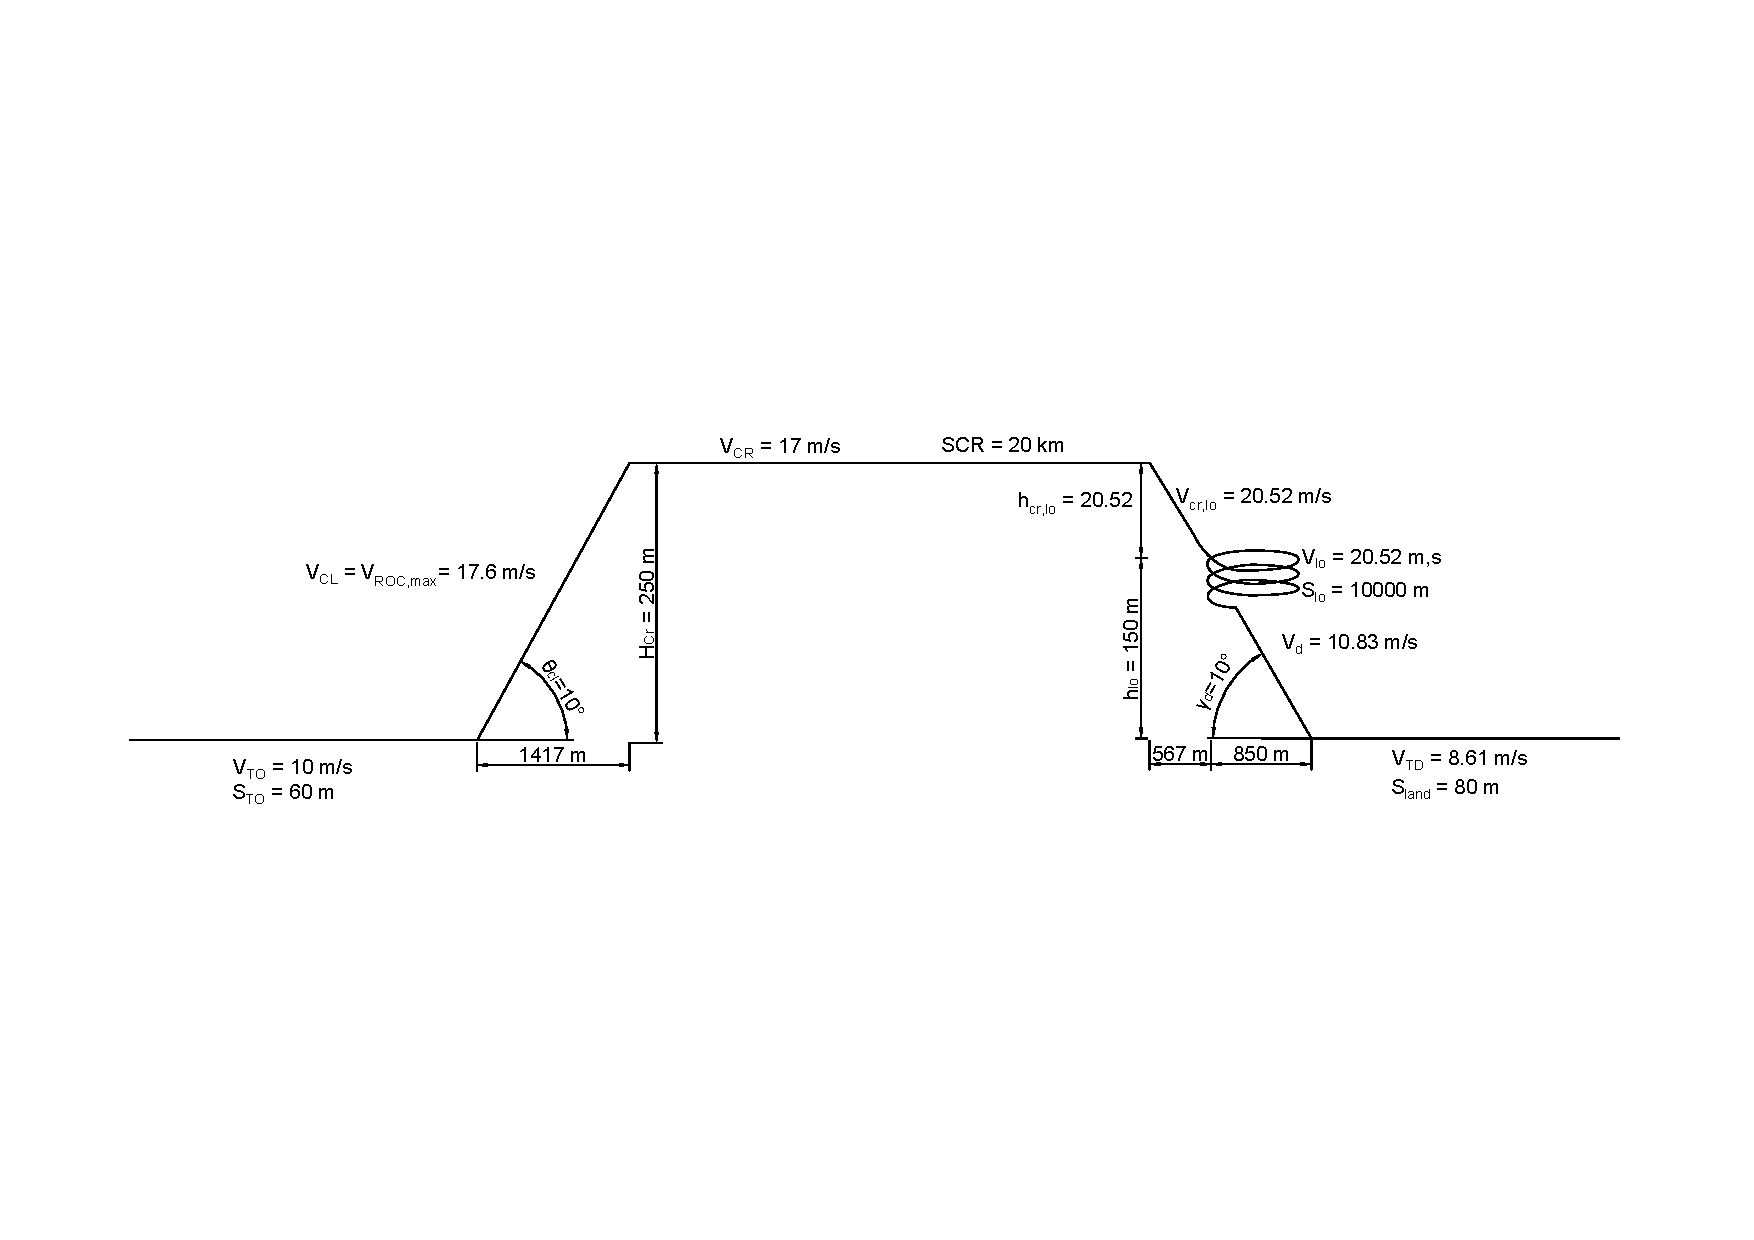
\includegraphics[width = \linewidth]{Drawing1-Model_final.pdf}
    \caption{Mission Profile}
    \label{Mission Profile}
\end{figure}


\subsubsection{Ground run}
The ground run distance of approximately 60 meters indicates the runway length needed for the UAV to accelerate. The UAV achieves the necessary airspeed for lift-off with an estimated takeoff velocity of 10 m/s. These parameters signify the aircraft's ability to transition from ground movement to flight efficiently. Such performance metrics are crucial for operations in constrained or limited-space environments. Overall, these values underscore the UAV's agility and suitability for diverse mission requirements \cite{EgglestonUnknownTitle2015}

$$ (V_{TO})_{_{Bricans \: Td100}} = 19 \: m/s$$
$$ (W_{TO})_{_{Bricans \: Td100}} = 22.67 \: kg$$

Since $ V_{TO} \: \alpha \: \sqrt{W_{TO}} $ for given $C_L$ , S (applicable for initial estimate)

$$ (V_{TO})_{_{des}} = (V_{TO})_{_{Bricans \: Td100}} \times \sqrt{\frac{(W_{TO})_{_{des}}}{(W_{TO})_{_{Bricans \: TD \: 100}}}} $$

$$ = 19 \times \sqrt{\frac{5.6 \times 9.81}{22.67 \times 9.81}} = 9.94 \: m/s \approx 10 \: m/s $$

\subsubsection{Climb} 
\cite{1000_questions}describes that the UAV will climb at an estimated velocity of 17.6 m/s to an operating altitude of 250 m AMSL. The rate of climb is about 3.06 m/s. Time spent here: 81.7 s

Calculation :- 
$$ (V_{TO})_{_{des}} = 10 \: m/s \Rightarrow (V_{stall})_{_{des}} = \frac{(V_{TO})_{_{des}}}{1.2} = 8.33 \: m/s $$
$$ (V_{md})_{_{des}} = 1.6 \times V_{stall} = 13.33 \: m/s $$
$$ (V_{ROC})_{_{max}} = 1.32 \times V_{md} = 17.6 \: m/s $$

\subsubsection{Cruise }
\cite{alhajjaji2017design} states that the UAV is tasked with conducting aerial surveillance and environmental monitoring, specifically targeting areas afflicted by plastic and solid waste accumulation. Operating at an estimated cruise speed of 17 m/s, it covers a range of 20 km. The UAV diligently surveys the designated areas throughout its mission duration, lasting 1176 seconds, utilizing its efficient speed and range capabilities to monitor and assess environmental conditions thoroughly.

\subsubsection{Descent to Mission Height}
The UAV will descend to an altitude of 150 m AMSL to study air quality at a sinking speed of 12.92 m/s for a 5 km range. Time spent here is 28 s.

Calculation: - 
$$(V_{cr,lo})_{_{design}} = 0.76 \times (V_{cr})_{_{des}} \;  (initial \: estimate) $$
$$ = 12.92 \: m/s $$

\subsubsection{Descent to land }
The UAV will descend at an estimated velocity of 10.13 m/s. To close ground proximity, the UAV gradually decelerates to an estimated touchdown velocity of 8.61 m/s. Time spent here is 80 s. By using formulas from \cite{Anderson1},
Calculation: - 
$$(V_des)_{_{design}} = (V_{mg})_{_{design}} = (V_{mg})_{_{design}} \times 0.76 = 10.13 \: m/s $$

\subsubsection{Landing run}
The landing ground run distance is approximately 80 metres, and the estimated touchdown velocity is 8.61 m/s.

Calculation: - 
$$ (V_{TD})_{_{design}} = 0.85 \times (V_{des})_{_{design}} = 8.61 \: m/s  $$
$$ \text{Vertical component of } (V_{TD})_{_{design}} = 8.61 \times \sin{10^{\circ}} $$
$$ = 1.495 \: m/s \leq 4 \: m/s \; \text{(For smooth landing)} $$


\begin{figure}
    \begin{subfigure}{.4\textwidth}
        \centering
        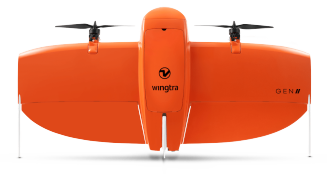
\includegraphics[width = 0.5\linewidth]{Aircraft pics/WingtraOne.png}
        \caption{Wingtraone}
        \label{Wingtra one}
    \end{subfigure}
    \begin{subfigure}{.4\textwidth}
        \centering
        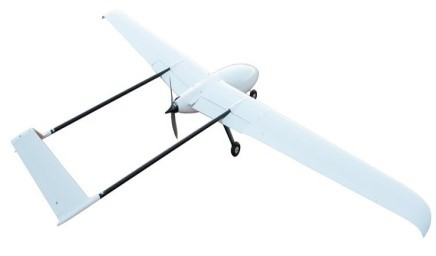
\includegraphics[width = 0.8\linewidth]{Aircraft pics/Albatross.jpg}
        \caption{Albatross}
        \label{Albatross}
    \end{subfigure}
    \begin{subfigure}{.4\textwidth}
    \centering
    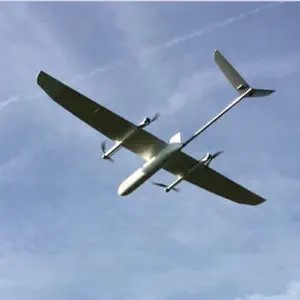
\includegraphics[width=0.9\linewidth]{Aircraft pics/Azimut.jpg}
    \caption{Azimut 2}
    \label{Azimut 2}
    \end{subfigure}
    \begin{subfigure}{.4\textwidth}
        \centering
        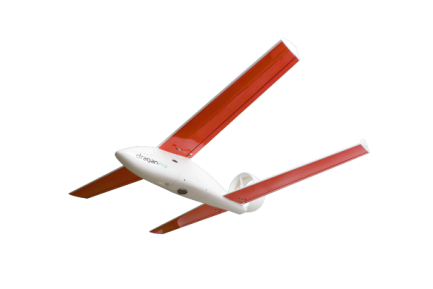
\includegraphics[width = 0.9\linewidth]{Aircraft pics/Dragonfly.png}
        \caption{Dragonfly Tango 2}
        \label{Dragonfly Tango 2}
    \end{subfigure}
    \begin{subfigure}{.4\textwidth}
        \centering
        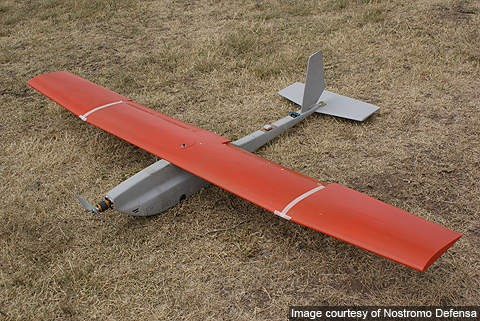
\includegraphics[width = 0.9\linewidth]{Aircraft pics/Nostroma.jpg}
        \caption{Nostroma Defensa Cadambra}
        \label{Nostromo Defence Cadambra}
    \end{subfigure}
    \begin{subfigure}{.4\textwidth}
        \centering
        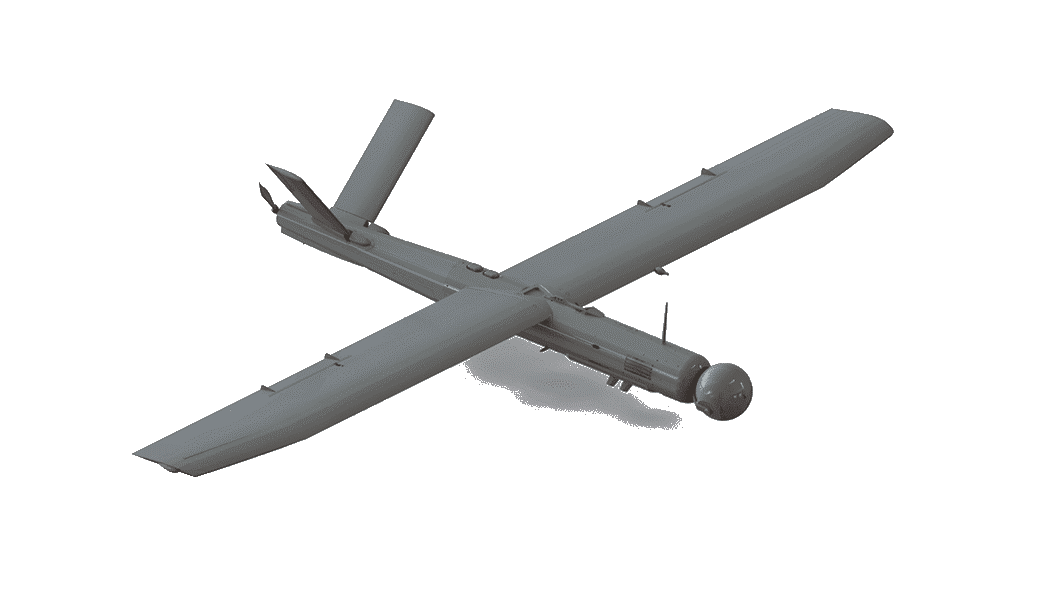
\includegraphics[width = 0.9\linewidth]{Aircraft pics/spylite.png}
        \caption{Spylite}
        \label{Spylite}
    \end{subfigure}
    \centering
    \begin{subfigure}{.4\textwidth}
        \centering
        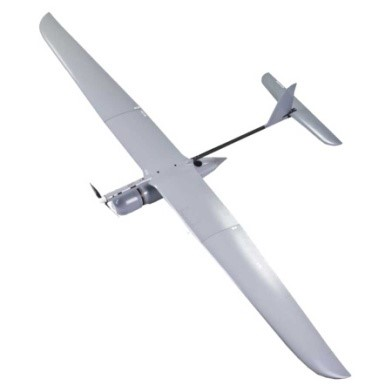
\includegraphics[width = 0.9\linewidth]{Aircraft pics/Skylark.jpg}
        \caption{Skylark}
        \label{Skylark}
    \end{subfigure}
    \caption{List of drones studied}
    \label{Drone pictures}
\end{figure}


\subsection{Data collection}

The data of all the parameters:-
% Please add the following required packages to your document preamble:
% \usepackage{graphicx}
\begin{table}[h]
\centering
\resizebox{\textwidth}{!}{%
\begin{tabular}{|c|c|c|c|c|c|c|c|}
\hline
SI no &
  UAV Name &
  \begin{tabular}[c]{@{}c@{}}MTOW \\ Kg\end{tabular} &
  \begin{tabular}[c]{@{}c@{}}Empty Weight\\ kg\end{tabular} &
  \begin{tabular}[c]{@{}c@{}}Battery Weight\\ kg\end{tabular} &
  \begin{tabular}[c]{@{}c@{}}Payload Weight\\ kg\end{tabular} &
  \begin{tabular}[c]{@{}c@{}}Range \\ km\end{tabular} &
  \begin{tabular}[c]{@{}c@{}}Endurance\\ min\end{tabular} \\ \hline
1 & Wingtraone   \cite{Wingtra}             & 4.5 & 2.387 & 0.604       & 1.509 &     & 59  \\ \hline
2 & Albatross    \cite{Albatross}             & 10  & 3.5   & 2.4         & 4.1   & 250 & 240 \\ \hline
3 & Azimut   2    \cite{Azimut}            & 9   & 2.5   & 2.8         & 3.7   &     &     \\ \hline
4 & Dragonfly   Tango 2  \cite{Dragonfly}      & 5   & 3     & 0.595+0.595 & 1.5   & 5   & 120 \\ \hline
5 & Nostromo   Defensa Cabure \cite{Nostromo} & 5   & 3.4   & 0.604       & 1     & 15  & 1.5 \\ \hline
6 & SPY   LITE    \cite{Bluebird}            & 9.5 & 4.5   & 1.5         & 1.35  & 80  & 240 \\ \hline
7 & Skylark I-LEX   \cite{Skylark}          & 7.5 & 5.5   & 0.8         & 1.2   & 40  & 180 \\ \hline
\end{tabular}%
}
\caption{Data part one}
\label{Data part one}
\end{table}


\newpage

\afterpage{\clearpage}


\textbf{\Huge{Chapter 2}}

\section{Preliminary Weight estimation}

Weight estimation is divided into various sections
\subsection{Payload weight estimation}
Rough estimate for payload
\begin{table}[h]
\centering
\resizebox{0.6\textwidth}{!}{%
\begin{tabular}{|c|c|}
\hline
Purpose                            & Weight \\ \hline
Camera                             & 492 g  \\ \hline
Sensor module                      & 520 g  \\ \hline
Bulk Tolerance (Wiring, Actuation) & 388 g  \\ \hline
Total Payload Estimate             & 1400 g \\ \hline
\end{tabular}%
}
\caption{Payload weight estimate}
\label{Payload weight}
\end{table}

\hfill



\subsection{Empty weight estimation}
The empty weight is the weight of the UAV without the battery and the payload, essentially the structural weight of the UAV. 
This is the first weight calculation in the Design process. \\

\begin{figure}[h]
    \centering
    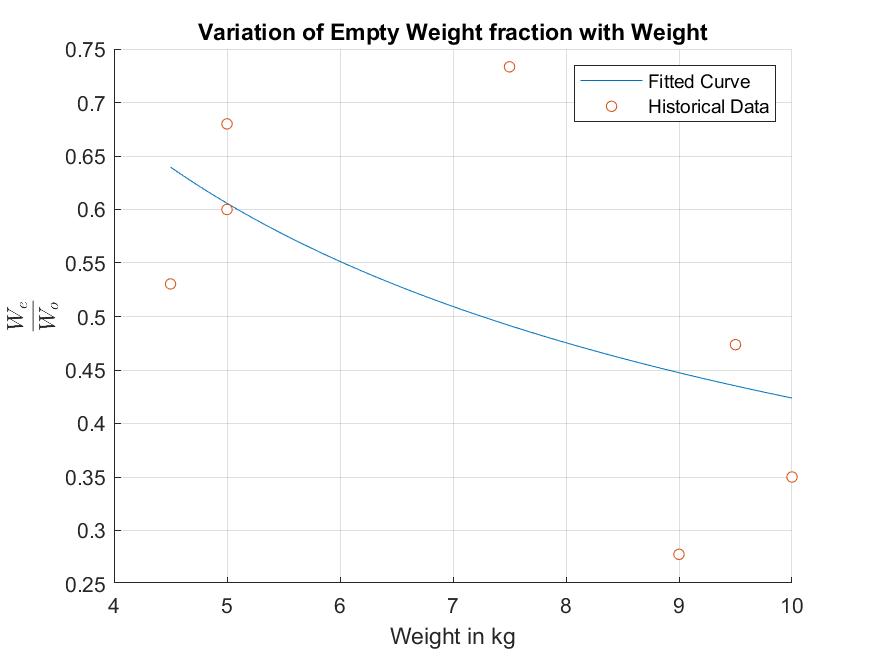
\includegraphics[width = 0.8\linewidth]{Codes/Week 2/Empty_weight.png}
    \caption{Empty weight estimation}
    \label{Empty Weight estimation}
\end{figure}


The process of estimating the empty weight ratio of a UAV involves fitting data into a mathematical curve using the equation $y = A x^c$, where A and C are variables. In this case, after conducting a curve fit, the values obtained were A = 1.3887 and C = -0.5155. By applying this curve fit equation, the empty weight of the UAV was calculated to be 3.1746 kg. This method allows for a quantitative estimation of the structural weight of the unmanned aerial vehicle based on the data analysis and mathematical modeling

\newpage

\subsection{Battery weight estimation}

Calculating the battery weight for a UAV  involves optimizing its weight based on the mission profile to avoid carrying unnecessary dead weight. To estimate the battery weight accurately, the first step is to determine the total energy required for each primary phase of flight. This entails analyzing the energy consumption during different flight phases such as takeoff, climb, cruise, hover, and landing. By understanding the energy demands at each stage of the mission profile, designers can calculate the total energy needed for the entire flight. This information is crucial for selecting an appropriately sized battery that can provide the required energy without adding excessive weight to the uav, ensuring optimal performance and efficiency throughout the mission
.

\subsubsection{Cruise}
The power required for the cruise condition of a UAV is a critical parameter that ensures the aircraft maintains steady flight during this phase. In essence, during cruise, the UAV is in force equilibrium, where the thrust and drag forces are balanced. The thrust required for cruise at a specific airspeed follows the drag profile, ensuring that the total drag does not exceed the available thrust and and therefore, the power required for cruise is a crucial factor in determining the energy consumption and performance of the UAV during this phase of flight.
For steady level we have ,
$$ L = W \; \; , \; \; T = D$$

$$ W = \frac{1}{2} \rho V^2 S C_L $$
$$ C_L = \frac{W}{\frac{1}{2} \rho V^2 S}$$
So,
$$ C_D = C_{D_0} + \frac{C_L^2}{\pi e AR} $$
Now 
$$ P = T\times V = D\times V $$

So, 
$$ P_R = \frac{1}{2}\rho V^3 S C_{D_o} + \frac{2 W^2}{ (\rho V S) \pi e AR} $$

$$P_R = f(W,\rho,V,C_{D_o},S,e,AR)$$

Taking approximations and inputting mission profile conditions

$$ P_R = f(W) $$

We will consider the Loitor phase as a cruise, too.

For our cruise phase of 17 m/s, we will need a power of 84.35 W 

\subsubsection{Climb }
The power required for climb in a UAV is the energy needed to ascend vertically, considering factors like climb rate, airspeed, weight, and propulsion efficiency. It determines the additional power required to overcome gravity during ascent, optimizing performance and energy efficiency for climbing phases of flight.
The power required for the climb is given by 
$$ P = W \times R.O.C + P_R $$

During the climbing phase of flight, a significant amount of power is required to ascend vertically. In our case, for the estimated weight of the UAV, a preliminary power of 251 watts is needed to facilitate a successful climb. This power allocation is essential to overcome gravity and achieve the desired ascent rate, ensuring efficient and effective performance during the climbing segment of the UAV's flight.

\subsubsection{Descent}
The power required for descent is 
$$ P = P_R - W \times Rate\: of\: descent$$
To prevent negative power estimates, we include an extra allowance in our calculations to ensure power never drops below zero. This buffer safeguards against unexpected power variations, guaranteeing the UAV always has sufficient power for optimal performance during flight

\subsubsection{Take off and Landing}
The Segments of takeoff and Landing do not take that much time. Also, estimating the energy spent in takeoff and landing is more complicated due to the need for carrying power. So, we will take an excess power of 20 percent to account for the errors in different power situations.

\subsubsection{Battery type selection \cite{Lipobattery}}
We will use a lithium polymer battery for our aircraft. Some of the advantages offered by a lithium polymer battery are that it is less likely to leak away and still rivals Lithium-ion batteries in terms of energy density. It is bulkier by volume, but by weight, it is comparable.

\begin{figure}[h]
    \centering
    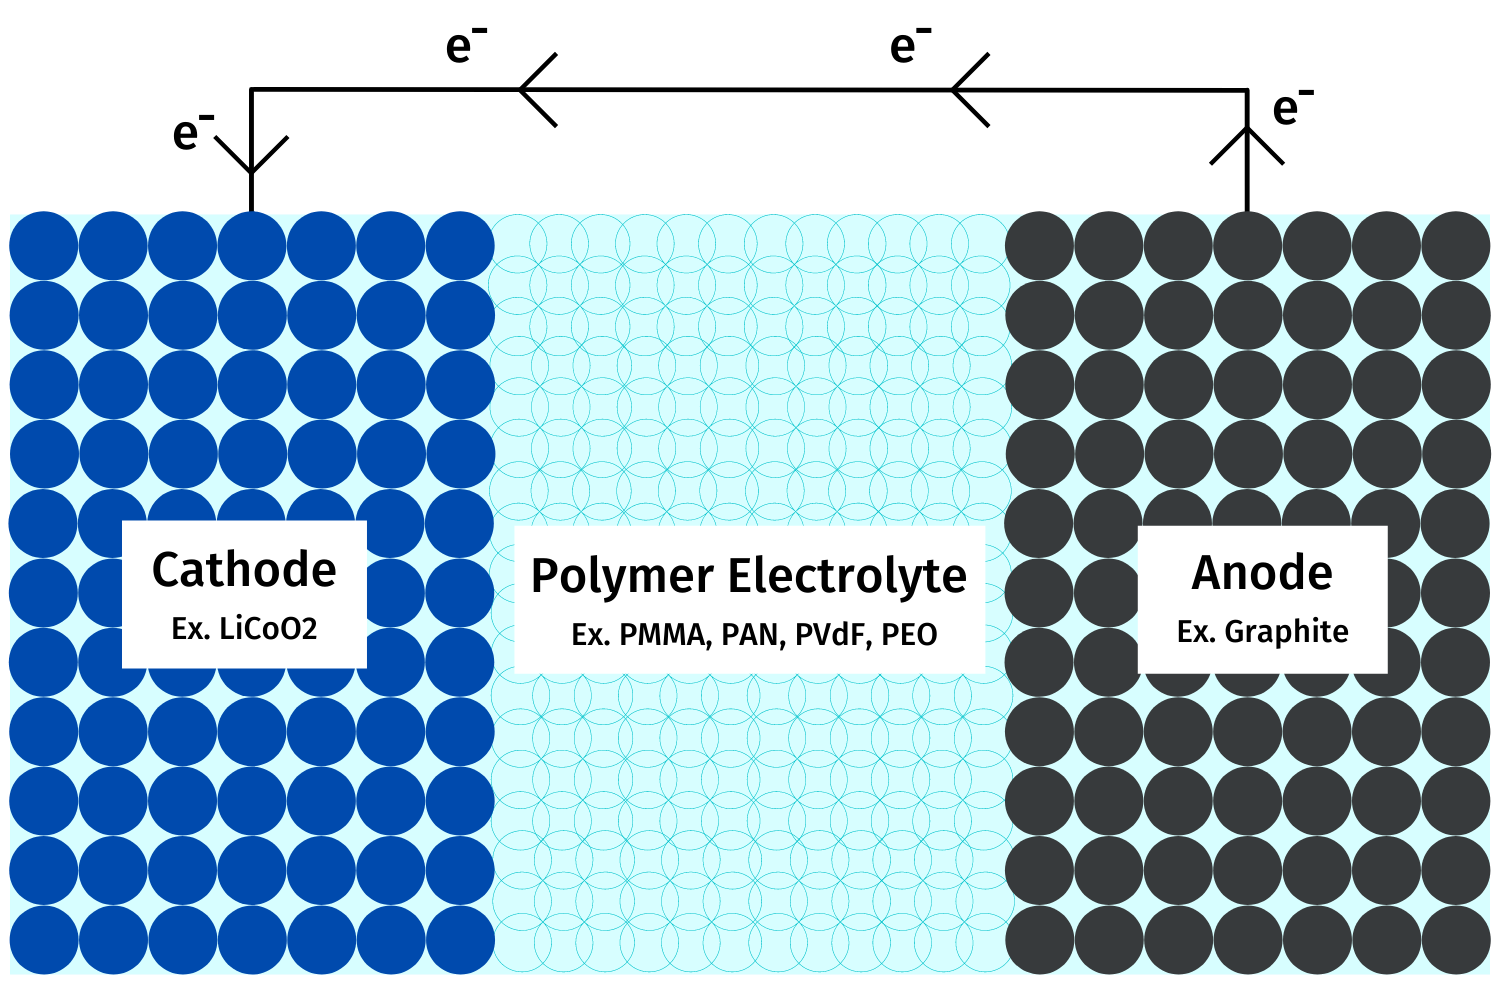
\includegraphics[width=0.5\linewidth]{Extra pics/LiPo_battery_diagram.png}
    \caption{Lithium Polymer battery}
    \label{Lithium Polymer battery}
\end{figure}

Lithium Polymer batteries are rechargeable batteries that transmit electricity due to the charge difference between the battery's Cathode and Anode parts. While pretty safe to handle, care should be taken not to get the battery near any fore source, or else it tends to catch fire.

We can estimate the energy in a battery by using this formula \cite{Lipobattery}:-

$$ \text{Battery Capacity} = \sigma \times \text{M}_\text{battery} $$

We used a commercially available battery to calculate the battery energy density of it \cite{Batteryref}. The energy density came out to be 237600 J/kg.

\subsubsection{Battery weight}

We can calculate the energy by multiplying the power required by the time spent in that phase. From energy, we can get battery weight by dividing it by energy density. 

In our case, the battery weight came out to be 0.933 kg.

%For lithium polymer batteries, the energy density is around 273600.

\subsection{Total weight estimation}

The total weight is given as:- 
$$ W_0 = W_{pl} + W_{e} + W_{f} $$
Where,
\begin{itemize}
    \item[-] $W_0$ is the total design weight.
    \item [-] $W_{pl}$ is the payload weight.
    \item [-] $W_{e}$ is the empty weight.
    \item [-] $W_{f}$ is the fuel weight (Battery in our case).
\end{itemize}

It can be transformed into:- 
$$W_{0} = \frac{W_{pl}}{1 - \frac{W_{e}}{W_{0}} - \frac{W_{f}}{W_0}}$$

If we have an initial approximation, we can run an iteration algorithm to determine the design weight when we keep the empty weight ratio as a variable.

%Generally, we take an initial estimate to be four times the payload weight. Correct initial weight is essential, or the code may blow up.

In our case, we use a special algorithm to preserve the momentum of the descent from the previous iteration. This is done because otherwise, the code will blow up and reach a negative value. 

$$ W_o = W_{\text{Previous iteration}} + W_{\text{New iteration}} $$

The code for the algorithm is mentioned below in the GitHub reference.

In our case, the design weight was 6.6102 kg after taking a 20 percent leverage over the original weight.

\begin{figure}
    \centering
    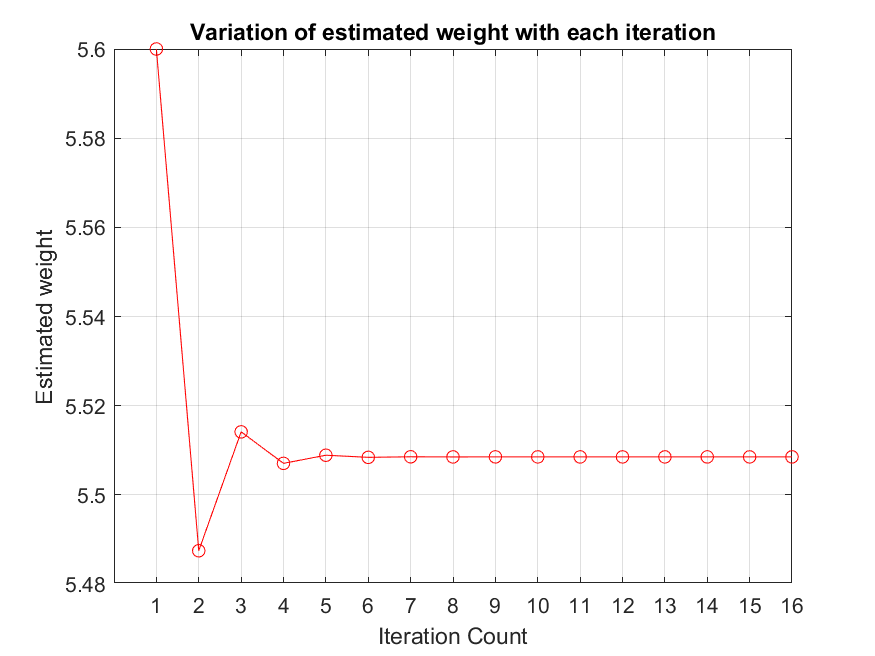
\includegraphics[width=0.75\linewidth]{Codes/Week 2/weight.png}
    \caption{Weight Estimation}
    \label{Weight Estimation}
\end{figure}

\vfill

\afterpage{\clearpage}

\newpage

\textbf{\Huge{Chapter 3}}

\section{Powerplant and Motor Selection}

\subsection { Aerodynamic Efficiency ${(L/D)}$}
The ratio of Lift-to-Drag is an indication of the aerodynamic efficiency of the airplane. An airplane has a high L/D ratio if it produces a large amount of lift or a small amount of drag. There are few peculiar L/D ratios that correspond to certain flight operating conditions of importance such as at minimum drag, minimum power, maximum range and so on.

\subsection { Calculation of Maximum Aerodynamic Efficiency ${(L/D)}_{max}$}
Because under cruise conditions lift is equal to weight, a high lift aircraft can carry a large payload. And because under cruise conditions thrust is equal to drag, a low drag aircraft requires low thrust. Hence, it is clear that L/D ratio of an aircraft operating in cruise corresponds to Maximum Lift-to-Drag ratio ${L/D}_{max}$.

we are going to mostly use historical data The reason is that we cannot do anything better because we are at a stage in design where we cannot get the accurate value of this parameter because we have not even finalized the configuration. All we know is the type of the aircraft that we are designing.

there are certain thumb rules available one simple guideline is
as a function of the wing aspect ratio.

The subsonic value of ${(L/D)}$ is very strongly dependent upon the aircraft configuration.

In level flight, we go for a condition that lift is equal to weight and hence, the ${(L/D)}$ will depend based mostly on the D because the L is
almost constant.
for subsonic aircraft, there are 2 main components of the drag or D. One is the parasite or Zero lift drag which is a function of the wetted area of the aircraft and the other is the induced or lift dependent drag, which is a function of the wingspan because it is a function of
aspect ratio which is span square by area. 

if we want to get a handle on both these aspects, the span as well as the wetted area.
We should consider not just the aspect ratio, but the wetted aspect ratio. The wetted aspect
ratio AR wet is defined as the square of the span divided by the wetted area of the aircraft.
And the wetted area aspect ratio is a much better indicator of ${(L/D)_{max}}$
Raymer, in his textbook has given this example, it is a very nice example, which shows that
you could have a totally different shape, but you may have the same value of maximum LD.
So,if the wetted aspect ratio of if the velocity ratio of 2 aircraft is similar, we can expect them to have the same or similar (LD)max values.

\textbf{Wingspan}: It is the distance between the wingtips of the UAV.\\

\textbf{Mean aerodynamic chord}: It is the average of the chord lengths across the cross sections of the wings.\\



The aspect ratio ($AR$) of a rectangular wing aircraft is calculated using the formula:
\[
AR = \frac{{\text{Wingspan}}}{{\text{Mean aerodynamic chord}}}\]
where the wingspan is the distance between the wingtips and the Mean aerodynamic chord is the average chord length of the wing.\\
By using steady-level conditions, where Lift = Weight, we have calculated the Lift Coefficient at cruise conditions.\\
When the lift force ($L$) of an aircraft equals its weight ($W$), the coefficient of lift ($C_L$) can be calculated using the formula:

\[
C_{L_{cruise}} = \frac{W}{\frac{1}{2} \times \rho \times V^2 \times S_{\text{ref}}}
\]
where $\rho$ is the density of air, $V$ is the velocity of the aircraft, and $S_{\text{ref}}$ is the reference wing area.
\subsubsection{Sample calculation of Aspect ratio and Lift Coefficient for cruise condition of Wingtraone UAV}
From the data collection done in week 2, we have estimated cruise velocity for our UAV as $V_{cruise}$ = 16m/s
\begin{itemize}
  \item Wingspan ($b$) = 125 cm (obtained from data collection)
  \item Reference wing area ($S_{\text{ref}}$) = 5065 cm\textsuperscript{2} (estimated from image processing)
\end{itemize} 

To calculate the aspect ratio (AR) using the formula $AR = \frac{b^2}{S_{\text{ref}}}$:

\[
AR = \frac{125^2}{5065} = \frac{15625}{5065} \ =  3.08
\]

So, the aspect ratio is 3.085.\\

Given:
\begin{align*}
    \text{Maximum Takeoff Weight (MTOW)} & = 44.15 \, \text{N} \\
    \rho & = 1.225 \, \text{kg/m}^3 \\
    S_{\text{ref}} & = 0.507 \, \text{m}^2 \\
    v_{\text{cruise}} & = 16 \, \text{m/s}
\end{align*}


For cruise conditions, we know that Lift = Weight.

{Calculating Coefficient of Lift for Cruise Conditions}

Estimation of $(L/D)_{\text{max}}$:

For steady cruise conditions, we know:

\begin{align}
\left(\frac{T}{W}\right)_{\min} &= \frac{1}{(L/D)_{\text{max}}} \tag{3.3} \\
\left(\frac{L}{D}\right)_{\text{max}} &= \sqrt{\frac{1}{\ 4CD_0 k}} = \sqrt{\frac{\pi e AR}{\ 4CD_0 k}} \tag{3.4}
\end{align}

Equation 3.3 has been used to determine $(L/D)_{\text{max}}$ for each of the aircraft. From Equation 3tovident that we need to determine $CD_0$ in order to obtain $(L/D)_{\text{max}}$.

Since it is Steady Cruise, the Equations of motion and aerodynamic relations are as follows:

\begin{align}
L &= W_0g \tag{3.5} \\
C_L &= \frac{2W_0g}{\rho V^2_{\text{cr}} c_r S_{\text{ref}}} \tag{3.6} \\
C_D &= CD_0 + kC_L^2 \tag{3.7}
\end{align}

Equation 3.6 is used to determine $C_L$ for each of the aircraft. Input parameters such as $V_{\text{cr}}$ (Velocity in cruise) and $S_{\text{ref}}$ vary for each aircraft. $V_{\text{cr}}$ is obtained for each aircraft during the data collection phase, and $S_{\text{ref}}$ is determined following the method stated in the above section.

For $(L/D)_{\text{max}}$:

$(L/D)_{\text{max}}$ and $AR_{\text{wet}}$ for each aircraft are obtained using Equations 3.4 and 3.3 respectively. The data obtained during this exercise is tabulated in Table 5.

Substituting the given values:
\[
C_{D0} = 0.1475 \times (0.556)^2
\]

Calculating \( C_{D0} \):
\[
C_{D0} \ = 0.1475 \times (0.556)^2 \ = 0.0461
\]

Therefore, the minimum drag coefficient is approximately \(0.0461\).\\
Now Let's calculate \( L/D_{\text{max}} \))
\begin{align*}
    k & = 0.1475 \\
    C_{D0} & = 0.046
\end{align*}

Equating lift to weight for cruise conditions:
\[
L = W
\]
\[
\frac{1}{2} \rho v_{\text{cruise}}^2 S_{\text{ref}} C_{L_{\text{cruise}}} = W_{\text{cruise}}
\]

Substituting the given values:
\[
\frac{1}{2} \times 1.225 \times 16^2 \times 0.507 \times C_{L_{\text{cruise}}} = 44.15
\]

Solving for $C_{L_{\text{cruise}}}$:
\[
C_{L_{\text{cruise}}} = \frac{44.15}{\frac{1}{2} \times 1.225 \times 16^2 \times 0.507} = 0.556
\]

For maximum lift-to-drag ratio (\( L/D_{\text{max}} \)):
\[
\frac{L}{D_{\text{max}}} = \frac{1}{2\sqrt{k \cdot C_{D0}}}
\]

Substituting the given values:
\[
\frac{L}{D_{\text{max}}} = \frac{1}{2\sqrt{0.1475 \cdot 0.046}}
\]

Calculating \( L/D_{\text{max}} \):
\[
\frac{L}{D_{\text{max}}} \ =  \frac{1}{2\sqrt{0.1475 \cdot 0.046}} = 6.103
\]

For minimum drag lift-to-drag ratio (\( L/D_{\text{minimum drag}} \)), it's the same as \( L/D_{\text{max}} \) due to the assumption that \( L/D_{\text{max}} = L/D_{\text{minimum drag}} \).

Therefore, both \( L/D_{\text{max}} \) and \( L/D_{\text{minimum drag}} \) are approximately \(6.103\).

\begin{table}[h]
\centering
\resizebox{\textwidth}{!}{%
\begin{tabular}{|c|c|c|c|c|c|c|c|}
\hline
SI no &
  UAV Name &
  \begin{tabular}[c]{@{}c@{}}MTOW \\ Kg\end{tabular} &
  \begin{tabular}[c]{@{}c@{}}Cruise speed\\ m/s\end{tabular} &
  \begin{tabular}[c]{@{}c@{}}$AR_{ref}$\end{tabular} &
  \begin{tabular}[c]{@{}c@{}}Wetted AR\end{tabular} &
  \begin{tabular}[c]{@{}c@{}}$C_{L}{cruise}$\end{tabular} &
  \begin{tabular}[c]{@{}c@{}}$\text{L/D}_{max}$\end{tabular} \\  \hline
1 & Wingtraone                & 4.5 & 16 & 3.085       & 1.874 &   0.556  & 6.103  \\ \hline
2 & Albatross                & 10  & 18.89   & 11.688         & 5.939   & 0.583 & 22.047 \\ \hline
3 & Azimut   2    & 9   & 13.89   & 5.776         & 2.992   & 0.690    &  9.198   \\ \hline
4 & Birdeye  600        & 8.5   & 20.57    & 8.948 & 4.474   & 0.452   & 21.772 \\ \hline
5 & Rafael Skylite BR & 8   & 30.56   & 9.969       & 5.145     & 0.608  & 18.024 \\ \hline
6 & Bluebird  Boomerang             & 9.5 & 22.12   & 5.948         & 3.118  & 0.640  & 10.219 \\ \hline
\end{tabular}
}
\caption{Data part two}
\label{Data part two}
\end{table}

\begin{figure}
    \centering
    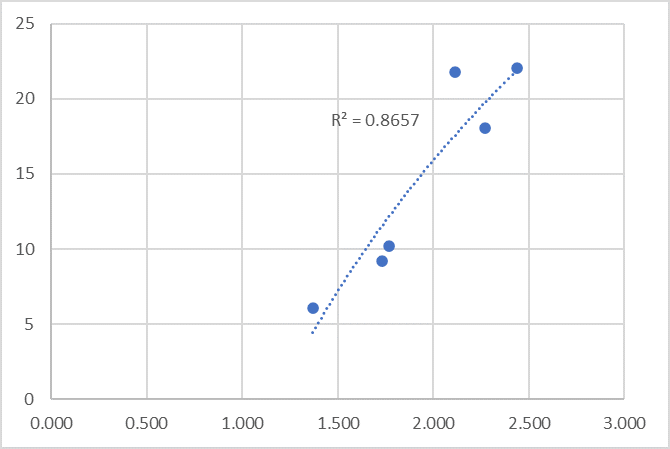
\includegraphics[width=0.8\linewidth]{graph.png}
    \caption{$\text{(L/D)}_{max}$ \text{v/s} $\sqrt{AR_{wet}}$ }
    \label{Data Collection}
\end{figure}

\newpage

\newpage
\newpage
\newpage
\newpage

\textbf{\Huge{Chapter 4}}

\section{Power Loading for Different mission segments}
The power loading for different mission segments of a UAV involves analyzing the power requirements during various phases of flight, such as take off, climb, cruise, and descent. This analysis helps in understanding the energy demands at different stages of the UAV's operation, aiding in the optimization of propulsion systems and energy management strategies for efficient and effective flight performance

 Given:
\begin{align*}
& L/D_{\text{max}} = 14.56067 \quad (\text{Taken from average of } L/D_{\text{max}} \text{ of data collection}) \\ 
& L/D_{\text{max}} = 30.249 \ln(\sqrt{AR_{\text{wet}}}) - 5.0483 \\
& \sqrt{AR_{\text{wet}}} = 1.912198 \\
& AR_{\text{wet}} = 3.6565 \\
& \frac{S_{\text{wet}}}{S_{\text{ref}}} = 1.9626 \quad (\text{From Data Collection and plotting graph between} \\
& \quad \text{ } \frac{S_{\text{wet}}}{S_{\text{ref}}} \text{ and } \sqrt{AR_{\text{wet}}}) \\
& AR_{\text{ref}} = \frac{b^2}{S_{\text{ref}}} = \left(\frac{b^2}{S_{\text{wet}}}\right) \left(\frac{S_{\text{wet}}}{S_{\text{ref}}}\right) = AR_{\text{wet}} \left(\frac{S_{\text{wet}}}{S_{\text{ref}}}\right) = 3.6565 \times 1.9626 = 7.175 \\
& e = 0.7 \quad (\text{for rectangular wing taken from NASA website}) \\
& k = \frac{1}{\pi e AR_{\text{ref}}} = \frac{1}{\pi \times 0.7 \times 7.175} = 0.063377 \\
& S_{\text{ref}} = 0.7 \text{ m}^2 \quad (\text{design requirement}) \\
& b = \sqrt{AR_{\text{ref}} S_{\text{ref}}} = 2.241098 \text{ m} \\
& c = \frac{b}{S_{\text{ref}}} = 0.312348 \text{ m} \\
& L/D_{\text{max}} = \frac{1}{2\sqrt{k C_{d0}}} \\
& C_{d0} = \frac{1}{4} \left(\frac{L}{D}\right)^2 k \\
& C_{d0} = 0.018606 \\
& \text{For NACA 4415 Airfoil:} \\
& C_{L_{\text{max, 2D}}} = 1.3393 \quad (\text{from airfoiltools.com}) \\
& C_{L_{\text{max, 3D}}} = 0.9 C_{L_{\text{max, 2D}}} = 1.2054 \\
& V_{\text{stall}} = 11.2 \text{ m/s} \quad (\text{design requirement}) \\
& V_{\text{stall}} = \sqrt{\frac{2(W/S)}{\rho C_{L_{\text{max, 3D}}}}} \\
& \frac{W}{S} = \frac{\rho V_{\text{stall}}^2 C_{L_{\text{max, 3D}}}}{2} \\
& \frac{W}{S} = 92.65865 \text{ N/m}^2 \\
\end{align*}
\subsection {Power Loading for Climb}
\textsc{}
\begin{align*}
& V_{\text{climb}} = V_{\text{minimum power}} = \sqrt{\frac{2W}{\rho S}} \left(\frac{k}{3C_{d0}}\right)^{\frac{1}{4}} \\
& V_{\text{climb}} = 12.69456 \text{ m/s} \\
& V_{\text{takeoff}} = 1.2 V_{\text{stall}} = 1.2 \times 11.2 = 13.44 \text{ m/s} \\
& S_{\text{rotation}} = V_{\text{rotation}} t_{\text{rotation}} = 13.44 \times 1.5 = 20.16 \text{ m} \quad (\text{ } t_{\text{rotation}} = 1.5 \text{ seconds for small airplanes - From JD Anderson}) \\
& R_{\text{rotation}} = 6.96 \times \frac{V_{\text{takeoff}}^2}{9.81} = 68.99719 \text{ m} \\
& \text{Climb angle} = \theta_{\text{c}} = \sin^{-1}\left(\frac{S_{\text{rotation}}}{R_{\text{rotation}}}\right) = 13.0995^\circ \\
& \text{ROC}_{\text{max}} = V_{\text{climb\_ROCmax}} \sin(\theta_{\text{c}}) = 12.6945 \sin(13.09915^\circ) = 2.8770757 \text{ m/s} \\
& \eta_{\text{prop}} \frac{P}{W} = \text{ROC}_{\text{max}} + \sqrt{\left(\frac{2(W/S) (k/3C_{d0})^{\frac{1}{2}}}{\rho}\right)^{\frac{1}{2}} \left(\frac{1.155}{(L/D)_{\text{max}}}\right)} \quad (\text{From JD ANDERSON}) \\
& \eta_{\text{prop}} \frac{P}{W} = 3.014397 \\
& \eta_{\text{prop}} = 0.8 \quad (\text{From JD Anderson}) \\
& \left(\frac{P}{W}\right)_{\text{climb}} = \frac{3.014397}{0.8} = 3.767996
\end{align*}
\subsection {Power Loading for Cruise}

\begin{center}
$V_{\text{cruise}} = 17 \, \text{m/s}$
\end{center}
\begin{align*}
\frac{T}{W}_{\text{cruise}} &= \frac{1}{(L/D)_{\text{cruise}}} = 0.068678 \\
\frac{P}{W}_{\text{cruise}} &= \frac{T}{W}_{\text{cruise}} \cdot V_{\text{cruise}} = 1.167529 \\
\frac{P}{W}_{\text{cruise}} &= 1.167529 \\
\end{align*}

\subsection {Power Loading for Descent}

\begin{center}
$V_{\text{approach}} = 14.56 \, \text{m/s}$ \\
$V_{\text{flare}} = 13.776 \, \text{m/s}$
\end{center}
\begin{align*}
\theta_{\text{descent}} &= \sin^{-1}\left(\frac{S_{\text{flare}}}{R_{\text{flare}}}\right) = 11.52162^\circ \\
V_{\text{cruise to descent}} &= V_{\text{cruise}} \cdot \cos(\theta_{\text{descent}}) = 16.65 \, \text{m/s} \\
V_{\text{average}} &= \frac{V_{\text{cruise to descent}} + V_{\text{approach}}}{2} = 15.605 \, \text{m/s} \\
D_{\text{descent}} &= D_{\text{cruise}} \cdot \cos(\theta_{\text{descent}}) = 4.520132 \, \text{N} \\
P_{\text{descent}} &= D_{\text{descent}} \cdot V_{\text{average}} = 70.53665 \, \text{W} \\
\end{align*}
\begin{center}
$\frac{P}{W}_{\text{descent}} = 1.087755$
\end{center}
\subsection {Power Required for Climb}

\begin{align*}
\frac{P}{W}_{\text{climb}} &= 3.767996 \\
P_{\text{climb}} &= \frac{P}{W}_{\text{climb}} \cdot W \\
&= 3.767996 \times 64.84 \\
&= 244.63 \, \text{W}
\end{align*}

\subsection {Power Required for Cruise}

\begin{align*}
\frac{P}{W}_{\text{cruise}} &= 1.167529 \\
P_{\text{cruise}} &= \frac{P}{W}_{\text{cruise}} \cdot W \\
&= 1.167529 \times 64.84 \\
&= 75.70 \, \text{W}
\end{align*}

\subsection {Power Required for Descent}
\begin{align*}
\frac{P}{W}_{\text{descent}} &= 1.087755 \\
P_{\text{descent}} &= \frac{P}{W}_{\text{descent}} \cdot W \\
&= 1.087755 \times 64.84 \\
&= 70.52 \, \text{W}
\end{align*}

\subsection {Power Required for Loiter}

Since we have assumed that loitering would be done in cruise conditions, we will take all cruise condition values and calculate the power required for loitering.

\begin{align*}
\frac{P}{W}_{\text{loiter}} &= 1.167529 \\
P_{\text{loiter}} &= \frac{P}{W}_{\text{loiter}} \cdot W \\
&= 1.167529 \times 64.84 \\
&= 75.70 \, \text{W}
\end{align*}
\subsection{Total Power Requirement}

The total power requirement encompasses the cumulative power demands for climb, cruise, descent, and loiter phases of the UAV's operation:

\[
\text{Total Power Requirement} = P_{\text{climb}} + P_{\text{cruise}} + P_{\text{descent}} + P_{\text{loiter}}
\]
\[
= 244.63 \, \text{W} + 75.70 \, \text{W} + 70.52 \, \text{W} + 75.70 \, \text{W} = 466.55 \, \text{W}
\]

To accommodate potential variations and ensure operational reliability, a tolerance of 20\% is applied to the total power value:

\[
\text{Adjusted Total Power } = 466.55 \, \text{W} + (0.20 \times 466.55 \, \text{W}) = 466.55 \, \text{W} + 93.31 \, \text{W} = 559.86 \, \text{W}
\]

Hence, the finalized total power requirement for the UAV, accounting for the specified tolerance, amounts to \textbf{ 559.86  \text{W}. }




\subsection {UAV powerplant selection}

\subsubsection {Battery Capacity Calculation}

For each mission segment, we will calculate the energy required in watt-hours by multiplying the power needed for that segment by its endurance time in hours.

\begin{itemize}
    \item Endurance for climb = 2 minutes = 0.0333 hours
    \item Endurance for cruise = 12 minutes = 0.2 hours
    \item Endurance for loiter = 10 minutes = 0.1667 hours
    \item Endurance for descent = 2 minutes = 0.0333 hours
    \item Endurance for takeoff and landing = 4 minutes = 0.0667 hours
\end{itemize}

\begin{align*}
\text{Energy for climb} &= P_{\text{climb}} \times \text{Endurance for climb} \\
&= 244.63 \times 0.0333 \\
&= 8.15 \, \text{Wh} \\[10pt]
\text{Energy for cruise} &= P_{\text{cruise}} \times \text{Endurance for cruise} \\
&= 75.70 \times 0.2 \\
&= 15.14 \, \text{Wh} \\[10pt]
\text{Energy for loiter} &= P_{\text{loiter}} \times \text{Endurance for loiter} \\
&= 75.70 \times 0.1667 \\
&= 12.61 \, \text{Wh} \\[10pt]
\text{Energy for descent} &= P_{\text{descent}} \times \text{Endurance for descent} \\
&= 70.52 \times 0.0333 \\
&= 2.35 \, \text{Wh} \\[10pt]
\text{Energy for takeoff and landing} &= (\text{Total power required} \times 0.20) \times \text{Endurance of takeoff and landing} \\
&= (559.86 \times 0.20) \times 0.0667 \quad \text{(We take 20 \% buffer of total power)} \\
&= 7.47 \, \text{Wh}
\end{align*}

The total energy required is the sum of energies for all mission segments:

\[
\text{Total Energy Required} = 8.15 + 15.14 + 12.61 + 2.35 + 44.45 = 82.7 \, \text{Wh}
\]

To calculate battery capacity, we'll use the formula:

\[
\text{Capacity (mAh)} = \frac{\text{Energy Required (Wh)}}{\text{Voltage (V)}} \times 1000
\]


Now, let's assume a typical lithium-ion battery voltage of 14.8V for calculation purposes.

\begin{align}
\text{Battery Capacity} &= \frac{45.72}{14.8} \times 1000 \\
& = 3089.18 \, \text{mAh}
\end{align}

So, the total battery capacity required for the aircraft is \textbf{3089.18 mAh}.

\subsubsection{Battery and Motor Selection}

\subsubsection{Battery Selection}

To meet the power requirements with a tolerance of about 1000 mAh, we have selected a MaxAmps Lithium Polymer (LiPo) battery with a capacity of 4000mAh operating at a voltage of 14.8V.

\begin{figure}[h]
    \centering
    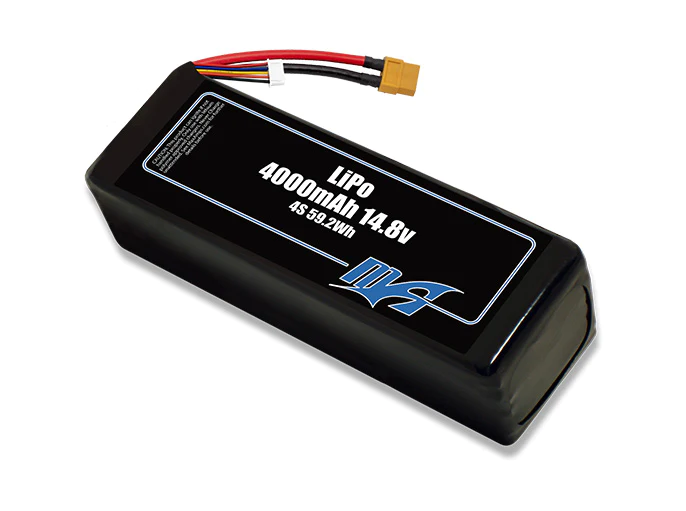
\includegraphics[width=0.7\textwidth]{LiPo-4000-4S-14.8v-Battery-Pack.jpg}
    \caption{LiPo Battery}
    \label{fig:battery}
\end{figure}

\begin{table}[h]
    \centering
    \caption{MaxAmps Lithium Battery Specifications}
    \begin{tabular}{|l|l|}
    \hline
    \textbf{Specification} & \textbf{Value} \\ \hline
    Brand & MaxAmps Lithium Batteries \\
    Capacity & 4000mAh \\
    Maximum Voltage & 16.8V \\
    Minimum Voltage & 12V \\
    Recommended Landing Voltage (Air) & 14V \\
    Recommended Cut-off Voltage (Ground) & 12.8V \\
    Chemistry & Lithium-Polymer (LiPo) \\
    Maximum Continuous Discharge & 128A \\
    Maximum Charge Current & 20A \\
    Watt Hours & 59.2Wh \\
    Energy Density & 151 Wh/kg \\
    Main Lead Length (Custom lengths available) & 5.5" (140mm) \\
    Balance Lead Length (Custom lengths available) & 5.5" (140mm) \\
    Length & 5.39" (138mm) \\
    Width & 1.85" (45mm) \\
    Height & 1.14" (48mm) \\
    Weight & 388g \\ \hline
    \end{tabular}
\end{table}

\subsubsection{Motor and Propeller selection}

We have selected AT 2317 Long Shaft KV 1440 Motor with APC 8x6 propeller to meet the above-calculated power requirements and voltage capacity. All the specifications are mentioned below.

Selecting the right propeller is crucial for efficient performance and optimal thrust generation. We have chosen an APC 8x6 propeller that is compatible with our motor.

\begin{figure}[h]
    \centering
    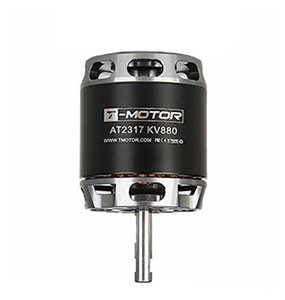
\includegraphics[width=0.3\textwidth]{motorr.jpg}
    \caption{AT2317 LONG SHAFT KV 1440 MOTOR}
    \label{fig:motor}
\end{figure}

\begin{figure}[h]
    \centering
    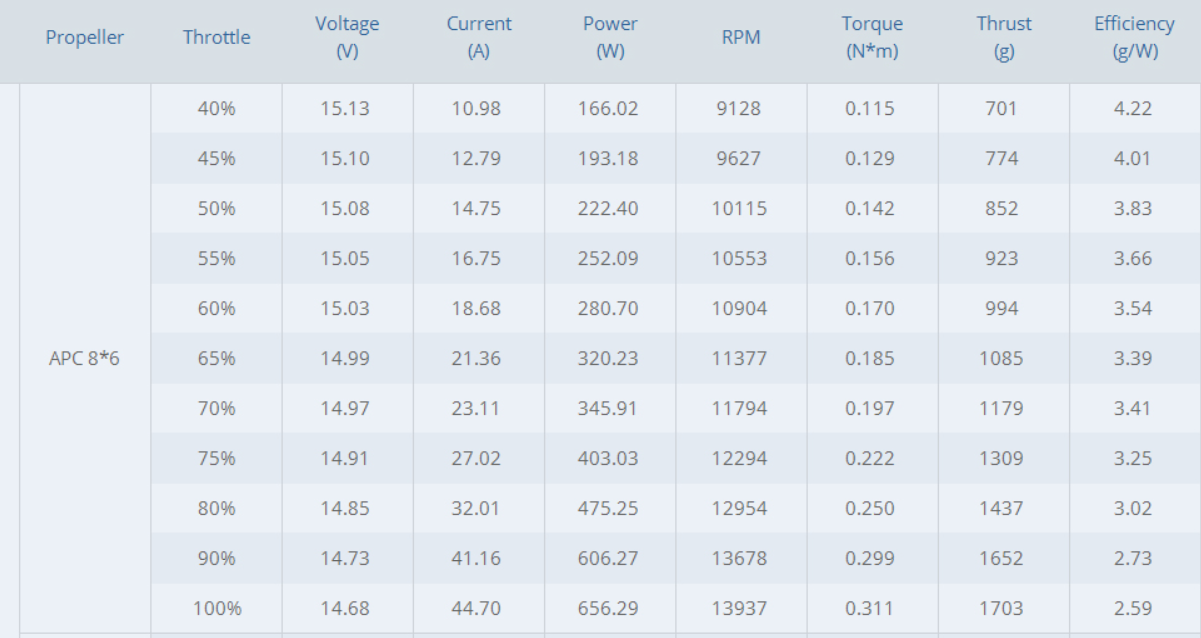
\includegraphics[width=0.8\textwidth]{motor specifications.png}
    \caption{MOTOR SPECIFICATIONS \cite{enginebuy}}
    \label{fig:motor_specifications}
\end{figure}

\begin{figure}[h]
    \centering
    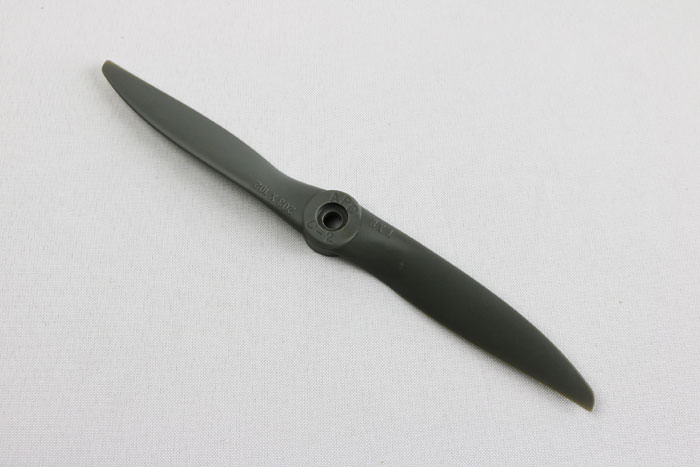
\includegraphics[width=0.5\textwidth]{propeller.jpg}
    \caption{APC 8x6 PROPELLER }
    \label{fig:propeller}
\end{figure}

\begin{figure}[h]
    \centering
    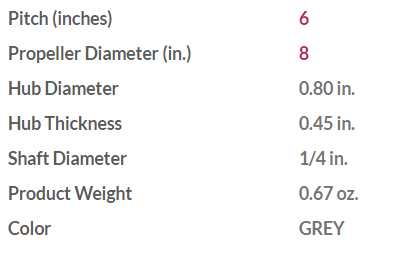
\includegraphics[width=0.6\textwidth]{propeller specifications.png}
    \caption{PROPELLER SPECIFICATIONS}
    \label{fig:propeller_specifications}
\end{figure}

\newpage

\clearpage
\begin{table}[h]
    \centering
    \caption{Powerplant Components and Weights}
    \label{tab:powerplant_weights}
    \begin{tabular}{|l|c|}
        \hline
        \textbf{Powerplant Component} & \textbf{Weight (g)} \\
        \hline
        Battery & 388 \\
        Motor & 80 \\
        Propeller & 19 \\
        \hline
    \end{tabular}
\end{table}


\textbf{\Huge{Chapter 5}}

\section{Wing Loading}

\subsection{Stall Criteria}
According to \cite{stall1}, Stall speed is the minimum speed at which the airplane remains controllable during its flight for a steady cruise. This is the point where the $C_L$ of the plane is maximum i.e. $C_{L_{\text{max}}}$

At this speed, the aircraft's Angle of attack becomes so large that the flow begins to separate at the top of the airfoil, resulting in a drop in lift if we increase the Angle of attack beyond that.

\begin{figure}[h]
    \centering
    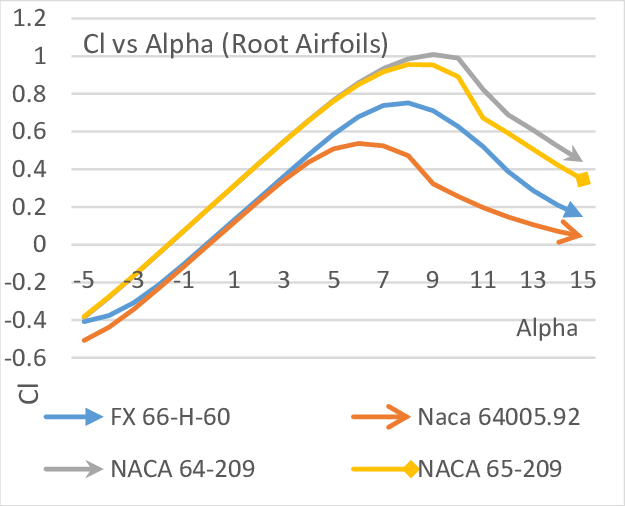
\includegraphics[width=0.4\linewidth]{Extra pics/Cllvsalpha.png}
    \caption{Variation of $C_L$ with angle of attack ref- \cite{stallpic}}
    \label{Variation of $C_L$ with angle}
\end{figure}

\subsection{ $\frac{W}{S}$ calculations }

\subsubsection{Stall}

According to our takeoff speed based on the Mission profile, which is ten m/s, we will take our stall speed to 8.33 m/s

At the stall, we know,
$$W = \frac{1}{2} \rho V^2 S C_{L_{max}} $$

So, $\frac{W}{S}$ comes out to be 107.5648 $N/m^2$. So, taking our estimated weight, the S comes out to be 1.0879 m.

%Since we are not dropping any payload or using any fuel, our $\frac{W}{S}$ will remain the same overall. However, in the case of turning, one wing can have a higher loading than the other to balance out forces. But the overall $\frac{W}{S}$ will remain the same.

\subsubsection{Take off parameter}

According to \cite{Raymer2006}, Raymer states that the Takeoff Parameter is given as:- 

$$\text{TOP} = \frac{\frac{W}{S}}{ \sigma C_{L_{TO}} \left( \frac{P}{W} \right) }$$
where,
\begin{itemize}
    \item[-] $\sigma$ is the density ratio we will take as 1.
    \item [-] $C_{L_{TO}}$ will be the Coefficient of lift at Takeoff 
\end{itemize}

We have taken the takeoff distance to 80 m, around 200 feet. Changing the previous equation:-

$$ \frac{W}{S} = \text{TOP} \times \sigma C_{L_{TO}} \left( \frac{P}{W} \right) $$

This equation will estimate the maximum $\frac{W}{S}$ we can take for our aircraft.

The TOP is given in ref \cite{Raymer. 2006} page number 130 in the form of a graph. The graph was digitalized using Image processing, and a Linear regression was taken in Figure:-\ref{Image processed Take off parameter}. 

We will take a power of 500 W for takeoff, which can be provided by out power-plant at 80 \% throttle. 

\begin{figure}[h]
    \centering
    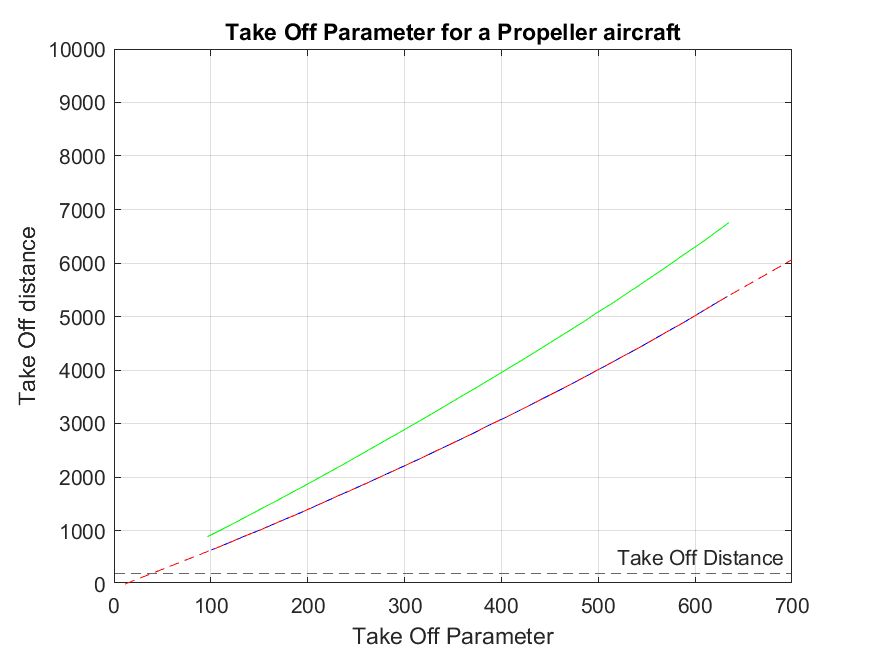
\includegraphics[width=0.8\linewidth]{Codes/Week 2/Takeoffparam.png}
    \caption{Image processed Take off parameter from \protect\cite{Raymer2006} pg no 130}
    \label{Image processed Take off parameter}
\end{figure}


We calculated that the maximum Wing loading during takeoff can be 352 $N/m^2$ for our case. This is sufficiently higher than the wing loading by Stall criteria, so we can rest assured that our plane can take off properly.

\subsubsection{Landing distance}

According to \cite{Raymer2006} Chapter 5.3.5, Raymer states that Landing distance is the minimum distance the plane will take to come to a halt.

It includes a clearing distance as well as a ground run distance. The landing distance heavily relies on $C_{L_{max}}$, which can be increased heavily by using flaps.

It is given as:- 
$$ S_{\text{Landing}} = 5*\left( \frac{W}{S} \right) \left( \frac{1}{\sigma C_{L_{\text{max}}}} \right) \: + \: S_a$$
where,
\begin{itemize}
    \item [-] $\sigma$ is the density ratio we will take as 1.
    \item[-] $C_{L_{\text{max}}} $ is the maximum Lift coefficient which we will take as 2 with flaps.
    \item[-] $S_a$ is the 'Clearance Distance' we should take before the actual ground roll to stay clear of all objects. We will take it as 50 m.
\end{itemize}

Using this, the Current landing estimate comes out to be 198.8 m, along with the Clearance distance. It should be noted that the distance can be significantly shortened by using flaps more efficiently to increase the maximum lift coefficient.

Also, some methods, like thrust reversion, can be considered in the design process to reduce landing distance.


\subsubsection{Cruise}

Raymer in \cite{Raymer2006} ch 5.3.7 discusses that for maximizing range in cruise, we would like a Wing loading, which is generally much higher than what is required for a wing required for stall speed. As a result, making a wing based on this estimate is pretty unsafe and will drastically increase stall speed.

The propeller aircraft will give us the maximum range when we have the highest L/D ratio. It is speed when the parasitic drag equals Induced drag as shown in Chapter 17 of \cite{Raymer. 2006}. Thus:-
$$qSC_{D_o} = qS\frac{C_L^2}{\pi e AR}$$
It will transform to give us:- 
$$ C_L = \sqrt{C_{D_o} \pi e AR }$$

This can be substituted back into the Cruise equation for the lift to get:-
$$ \frac{W}{S} = q \sqrt{C_{D_o} \pi e AR}$$
where, q is $\frac{1}{2} \rho V^2 $

For our cruise condition, our Wing loading comes out to be 95.91 $N/m^2$. This is expected for a perfect cruise, so having as small a wing as possible to minimize impossible drag.

\subsubsection{Loiter}

According to Raymer in CH 5.3.8 of \cite{Raymer. 2006} he states that the time of loiter will be most when the induced drag is three times the parasitic drag. 
$$C_L = 3 C_{D_o}$$

Assuming Loiter to be steady, we compute the wing loading as:-
$$\frac{W}{S} = q \sqrt{3C_{D_o} \pi e AR}$$
For our case, the optimal wing loading is 166.12 $N/m^2$.

Thus, We can infer that we must decrease our loiter speed to a low value to decrease the optimal wing loading in the next iteration. For example, for a loiter velocity of 15 m/s, we will get wing loading to be 130 $N/m^2$.

\subsection{Second weight estimate}

We got more accurate solutions of values from the previous values. 

From the Power loading, we got weight of the battery as well as the propeller and motor configuration. So when we input these values in the formula for the weight estimate, we get:- 

$$W_{0} = \frac{W_{pl}  +  W_{\text{battery}}+  W_{\text{Propeller}} + W_{\text{Motor}}}{1 - \frac{W_{e}}{W_{0}}}$$

Where:-
\begin{itemize}
    \item[-] $W_{\text{battery}}$ is battery weight which is 639 g.
    \item[-] $W_{\text{Propeller}}$ is propeller weight which is 19 g
    \item[-] $W_{\text{Motor}}$ is Motor weight which is 150 g.
    \item[-] $\frac{W_{e}}{W_{0}}$ is the empty weight fraction from initial estimate.
\end{itemize}

\begin{figure}[h]
    \centering
    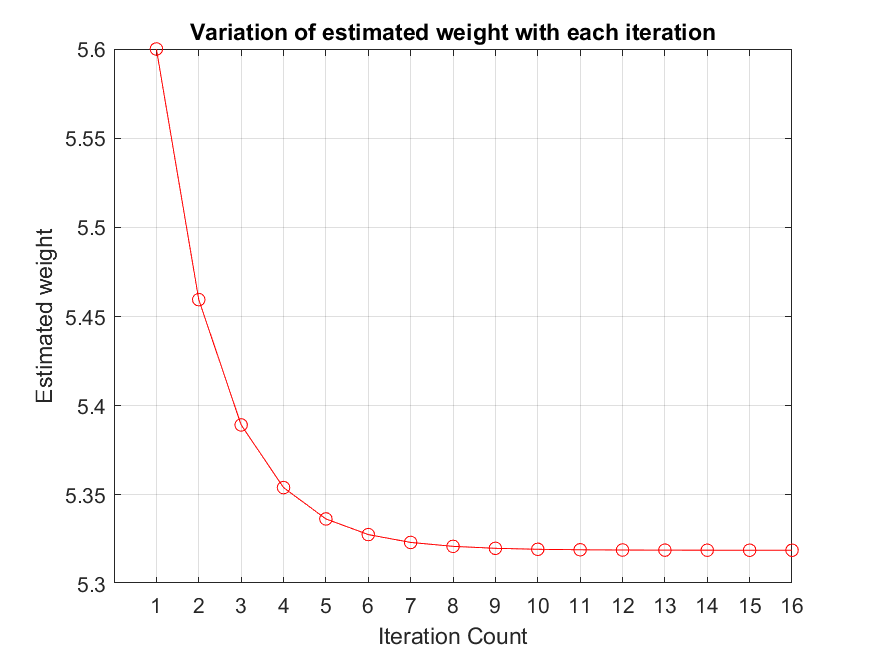
\includegraphics[width=1.0\linewidth]{Codes//Week 2/weight_2.png}
    \caption{Second weight estimate iteration}
    \label{Second weight estimate iteration}
\end{figure}

According to our new estimate, the weight after tolerance is 6.38 kg.

\afterpage{\clearpage}
\newpage

\textbf{\Huge{Chapter 6}}
\section{Wing Design}
This section estimates the Lift Coefficient for the cruise phase in the UAV mission profile. Various airfoils are evaluated using data from reputable airfoil databases, followed by simulations conducted through the XFLR5 software. We scrutinize performance diagrams and explore multiple wing configurations, factoring in various design parameters such as chord length, span length, high lift devices (e.g., flaps), taper ratio, and sweep Angle. Upon achieving performance plots closely aligning with our design specifications and considering practical feasibility, we finalize airfoil and wing configuration for representation.
\vspace{5mm} 
 

\color{red}
\subsection{\large Calculation of Design Lift Coeffient}

      \text{\large \underline{ Cruise}}

\color{black}
The pivotal phase in the mission profile is the Cruise Phase, where the mini UAV operates at an altitude of 100 meters with a velocity of 18 m/s. We aim to select a wing that demonstrates optimal aerodynamic performance during this phase, specifically by maximizing the Lift-to-Drag ratio at the desired operating Lift Coefficient for the cruise. Initially, we calculate the Lift Coefficient in cruise condition \\
Given:\\
 Cruise Velocity: \( v_{\text{cruise}} = 17 \) m/s\\
Density: \( \rho_{atm} = 1.225 \) kg/m³\\
 Takeoff weight: \( W_0 = 62.58 \) N\\
 Reference area: \(S = 0.7 m^2\) 

We can calculate the Lift Coefficient for the cruise using the formula:

\[
C_{L_{\text{cruise}}} = \frac{W_0}{\frac{1}{2} \rho_{atm} v_{\text{cruise}}^2 S}    \tag{6.1} \]

Thus, the lift coefficient for cruise is \( C_{L_{\text{cruise}}} = 0.5048 \). 
\color{red}
\subsection{Calculation of flow parameters}
\color{black}
Estimating flow parameters such as Reynolds number and Mach number for the cruise condition is essential in selecting the most suitable airfoil for our UAV. These parameters provide crucial insights into the aerodynamic behavior of the airfoil at the designated operating conditions, guiding the selection process toward optimal performance and efficiency. 
\color{red}
\begin{itemize}
\item{\underline{Reynolds number}}
\color{black}
\\Reynolds number is a crucial parameter in airfoil selection as it helps determine the aerodynamic behavior of the airfoil under different flow conditions. It is defined as the ratio of inertial forces to viscous forces within a fluid flow regime and is instrumental in predicting flow patterns around an airfoil. In airfoil selection, the Reynolds number provides insights into the transition from laminar to turbulent flow, which significantly impacts the aerodynamic performance and efficiency of the airfoil.

Given the parameters:

 Chord length (\( c \)): 0.312347524 m\\
 Cruise Speed (\( V_{\text{cr}} \)): 17 m/s\\
 Atmospheric Density (\( \rho_{\text{atm}} \)): 1.2256 kg/m³\\
 Atmospheric Viscosity (\( \mu_{\text{atm}} \)) at 15°C: \( 1.81 \times 10^{-5} \) Pa-s

The Reynolds number (\( Re \)) can be calculated using the formula:

\[
Re = \frac{V_{\text{cr}} \cdot c}{\nu_{\text{atm}}} \tag{6.2}
\]

Where \( \nu_{\text{atm}} \) is the kinematic viscosity and is given by \( \frac{\mu_{\text{atm}}}{\rho_{\text{atm}}} \).

Substituting the given values into the formula:

\[
Re = \frac{17 \times 0.312347524}{\frac{1.81 \times 10^{-5}}{1.2256}} \tag{6.3}
\]

\[
Re = 359548.24
\]

Therefore, the Reynolds number for the given parameters is \( 359548.24 \). 
\color{red}
\item{\underline {Cruise Mach Number}}
\color{black}
\\Cruise Mach number is a crucial parameter in airfoil selection as it characterizes the relative speed of the aircraft to the speed of sound in the surrounding air. It is defined as the ratio of the aircraft's velocity to the speed of sound in the medium. Understanding the cruise Mach number is vital in airfoil selection as it helps determine the aerodynamic behavior of the airfoil at high velocities, particularly in transonic and supersonic flight regimes.

Given the parameters:

 Specific heat ratio (\( \gamma \)): 1.4\\
 Air Gas Constant (\( R \)): 287.05287 J/kgK\\
 Atmospheric Temperature at Mean Sea Level (\( T_{\text{atm}} \)): 288.15 K\\
 Cruise velocity (\( V_{\text{cr}} \)): 17 m/s\\

The speed of sound (\( a \)) can be calculated using the formula:

\[
a = \sqrt{\gamma R T_{\text{atm}}} \tag{6.4}
\]
And the cruise Mach number (\( M_{\text{cr}} \)) can be calculated as:

\[
M_{\text{cr}} = \frac{V_{\text{cr}}}{a} \tag{6.5}
\]

Substituting the given values into the formulas:

\[
a = \sqrt{1.4 \times 287.05287 \times 288.15}  = 340.3 \, \text{m/s}
\]

\[
M_{\text{cruise}} = \frac{17}{340.3} = 0.0499 \tag{6.6}
\]

Therefore, the cruise Mach number for the given parameters is  0.0499.
\end{itemize}
\color{black}
\textbf{ \large The parameters below are guiding our airfoil selection.}
\begin{table}[h]
\centering
\begin{tabular}{ll}
\hline
Cruise Speed (m/s) & 17 \\
CL\_cruise & 0.5048 \\
Reynolds Number (Re) & 359,548.24 \\
Cruise Mach Number (M.cruise) & 0.049956804 \\
Maximum Lift-Drag Ratio (L/D)max & 14.56067 \\
\hline
\end{tabular}
\end{table}\\
\color{red}
\subsection{ Airfoil selection}

 \large \underline{SA7035 Airfoil}\\
\color{black}
We have selected the SA7035 airfoil for the above flow parameters, which is suitable for our UAV. The SA 7035 airfoil, developed by the German Aerospace Center (DLR), is highly favored in the UAV and light aircraft sectors for its exceptional aerodynamic properties. Renowned for its high lift-to-drag ratio and reliable stall behavior, it excels in various flight conditions, including cruising and maneuvering.

Featuring a thick profile and optimized camber distribution, the SA 7035 generates ample lift while keeping drag levels low, ensuring efficient performance, especially during extended cruise phases. Its forgiving stall characteristics also enhance safety and maneuverability, appealing to pilots of all skill levels.
\begin{figure}[h]
    \centering
    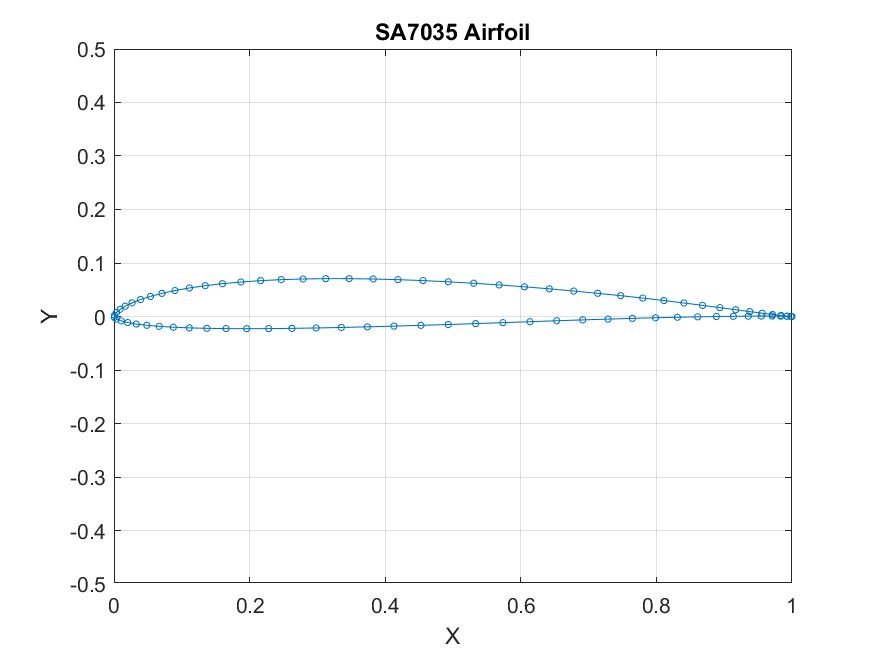
\includegraphics[width = 0.85\linewidth]{Codes/Week 6/Airfoil.png}
    \caption{SA7035 Airfoil}
    \label{SA7035 Airfoil}
    \end{figure}
\begin{table}[h]
\centering
\caption{SA7035 Airfoil Parameters}
\begin{tabular}{ll}
\hline
Max Cl/Cd & 71.2969 \\
$\alpha_{\text{maxCl/Cd}}$ & 5 deg \\
$C_{\text{Lmax}}$ & 1.2535 \\
$\alpha_{\text{Stall}}$ & 12.25 deg \\
Max thickness & 9.2\% at 27.9\% chord \\
Max camber & 2.4\% at 41.9\% chord \\
\hline
\end{tabular}
\end{table}
\newpage
We will now create graphs illustrating the relationship between Lift Coefficient ($C_L$) and Angle of Attack ($\alpha$), as well as the relationship between Drag Coefficient ($C_D$) and Angle of Attack ($\alpha$). We analyze these graphs to assess whether the airfoil meets the required performance criteria.
\newpage
\begin{figure}[H]
    \centering
     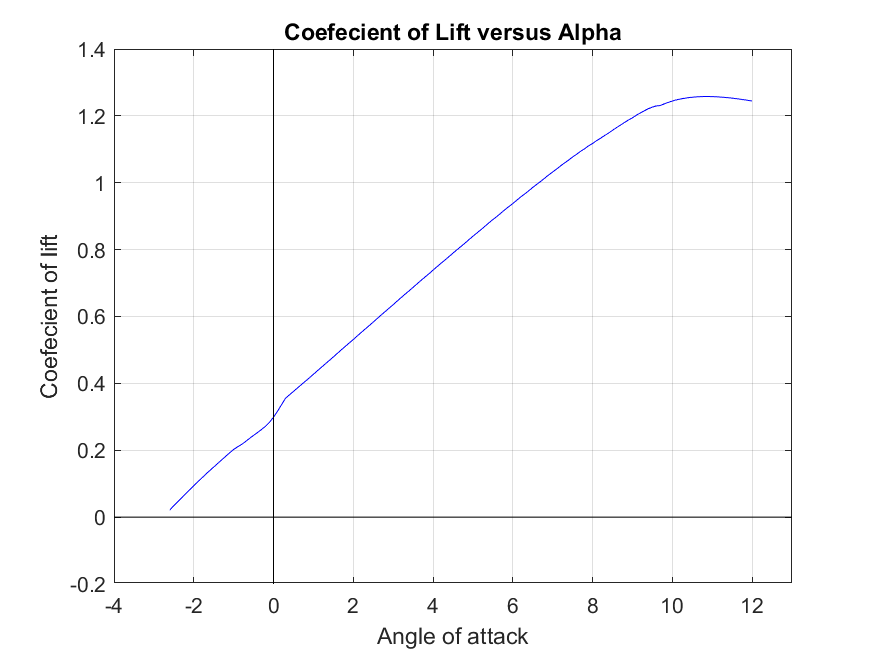
\includegraphics[scale = 0.8]{Codes/Week 6/Cl_alpha.png}
    \caption{Coefficient of lift vs Angle of attack}
    \label{Coefficient of lift vs Angle of attack}
\end{figure}

\begin{figure}[H]
    \centering
    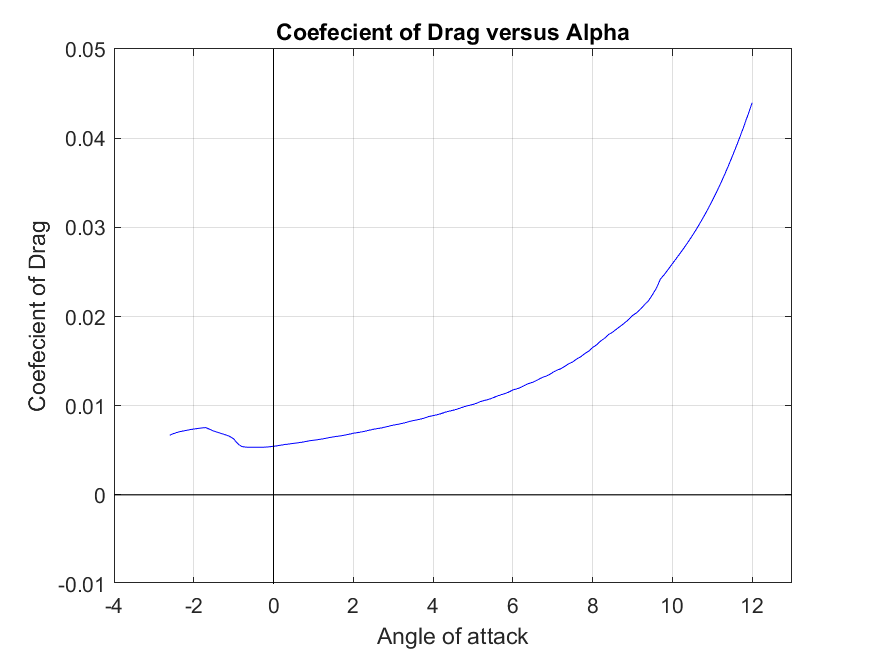
\includegraphics[scale = 0.8]{Codes/Week 6/Cd_alpha.png}
    \caption{Coefficient of drag vs Angle of attack}
    \label{Coefficient of drag vs Angle of attack}
\end{figure}

\begin{figure}[H]
    \centering
    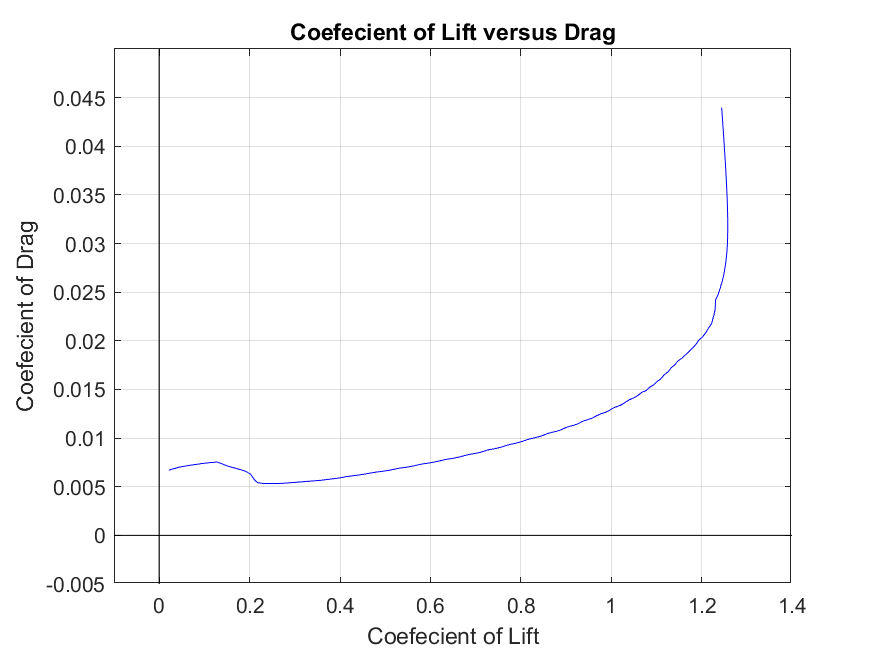
\includegraphics[scale = 0.8]{Codes/Week 6/Cl_Cd.png}
    \caption{Coefficient of lift vs coefficient of drag}
    \label{Coefficient of lift vs coefficient of drag}
\end{figure}

\begin{figure}[H]
    \centering
    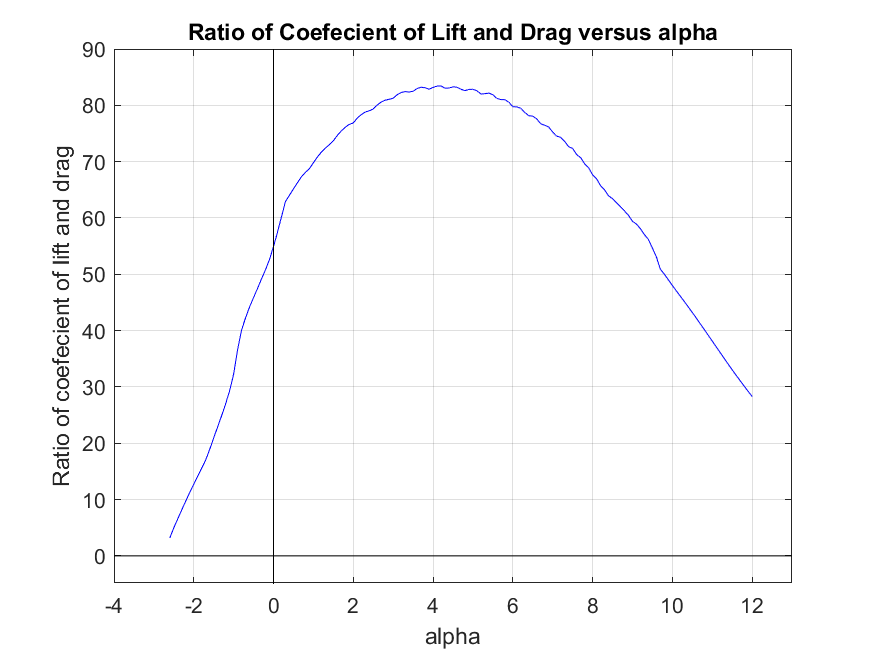
\includegraphics[scale = 0.8]{Codes/Week 6/Cl_Cd_ratio.png}
    \caption{Cl/Cd vs Angle of attack}
    \label{Cl/Cd vs Angle of attack}
\end{figure}
\newpage

We have established that the Lift Coefficient ($C_L$) during cruise conditions, which is 0.5048, is achieved at an angle of attack of 2.5 degrees. This value notably falls below the stall angle of attack, suggesting favorable performance attributes of the airfoil. Hence, this airfoil is considered preferable.

\color{red}
\subsection{Wing Configuration}

%\documentclass{article}


%\begin{document}

{\color{red}\textbf{Low-Wing Configuration:}}

{\color{black}
\textbf{\textcolor{red}{Advantages:}}
\begin{itemize}
  \item Enhanced stability: Low-wing UAVs exhibit better lateral stability during flight, making them well-suited for missions requiring precision control, such as surveillance and mapping.
  \item Payload capacity: Placing the wings beneath the fuselage allows for larger payload capacity, as payloads can be mounted directly underneath without wing interference.
  \item Aerodynamic efficiency: Low-wing UAVs may benefit from reduced interference drag between the wings and the fuselage, improving overall aerodynamic efficiency and potentially longer endurance.
  \item Ground operations: The low-wing configuration facilitates easier ground operations, including launching and landing, especially in confined spaces, as the wings do not obstruct ground clearance.
\end{itemize}

\textbf{\textcolor{red}{Disadvantages:}}
\begin{itemize}
  \item Vulnerability to ground debris: With the wings positioned beneath the fuselage, low-wing UAVs are more susceptible to damage from ground debris during takeoff and landing, which could potentially lead to damage to the wings or payload.
  \item Limited ground clearance: Low-wing UAVs may have limited ground clearance, which could pose challenges when operating on rough terrain or uneven surfaces.
  \item Visibility: While low-wing configurations offer good visibility for the payload, certain types of sensors or cameras mounted on top of the fuselage may experience slightly reduced visibility.
\end{itemize}
}

{\color{red}\textbf{Mid-Wing Configuration:}}

{\color{black}
\textbf{\textcolor{red}{Advantages:}}
\begin{itemize}
  \item Balanced lift distribution: Mid-wing UAVs typically achieve a balanced lift distribution, enhancing stability and control during flight maneuvers.
  \item Aerodynamic efficiency: Similar to low-wing configurations, mid-wing UAVs can benefit from reduced interference drag between the wings and the fuselage, contributing to overall aerodynamic efficiency.
  \item Visibility: Mid-wing designs provide good visibility for sensors and cameras mounted on the fuselage, allowing for effective surveillance and reconnaissance missions.
  \item Payload flexibility: The mid-wing configuration allows for flexible payload integration options, as payloads can be mounted on top of the fuselage without interference from the wings.
  \item Ground clearance: Mid-wing UAVs typically have sufficient ground clearance for landing gear and other components, making them suitable for various terrain conditions.
\end{itemize}

\textbf{\textcolor{red}{Disadvantages:}}
\begin{itemize}
  \item Complexity: Mid-wing configurations may involve more complex structural design and integration, especially when considering payload mounting and aerodynamic considerations.
  \item Maintenance accessibility: Accessing components on top of the fuselage, such as sensors or cameras, may require additional effort and time compared to configurations with lower wing wings.
  \item Vulnerability to damage: The mid-wing position exposes the wings to potential damage during ground operations, such as takeoff and landing, especially in rough terrain.
  \item Weight distribution: Achieving optimal weight distribution in mid-wing UAVs can be challenging, as the payload and other components need to be carefully balanced to maintain stability and performance.
\end{itemize}
}

{\color{red}\textbf{High-Wing Configuration:}}

{\color{black}
\textbf{\textcolor{red}{Advantages:}}
\begin{itemize}
  \item Excellent visibility: High-wing UAVs provide unobstructed visibility for sensors, cameras, and other payloads mounted beneath the fuselage, facilitating effective surveillance and reconnaissance missions.
  \item Stability: High-wing configurations typically offer excellent inherent stability, especially during banking maneuvers, making them suitable for various applications, including aerial mapping and monitoring.
  \item Protection from ground debris: With the wings positioned above the fuselage, high-wing UAVs are less susceptible to damage from ground debris during takeoff and landing, enhancing durability and reliability. Our payload module will also be safe.
  \item Payload flexibility: High-wing designs allow flexible payload integration options, as payloads can be mounted beneath the fuselage without wing interference.
  \item Ease of ground operations: High-wing UAVs often feature ample ground clearance, making takeoff and landing operations easier, especially in rough or uneven terrain.
\end{itemize}

\textbf{\textcolor{red}{Disadvantages:}}
\begin{itemize}
  \item Aerodynamic interference: High-wing configurations may experience increased interference drag between the wings and the fuselage, potentially impacting overall aerodynamic efficiency and endurance.
  \item Limited maneuverability: High-wing UAVs offer stability but may have slightly reduced maneuverability compared to other configurations, which can be considered for specific mission profiles.
  \item Weight distribution: Achieving optimal weight distribution in high-wing UAVs can be challenging, as the payload and other components must be carefully balanced to maintain stability and performance.
  \item Complexity in payload integration: Mounting specific
\end{itemize}
\vspace{5mm} 
By considering all the wing configurations, we have decided to go with\textbf{ high wing configuration} for our UAV.
\begin{figure}[H]
    \centering
    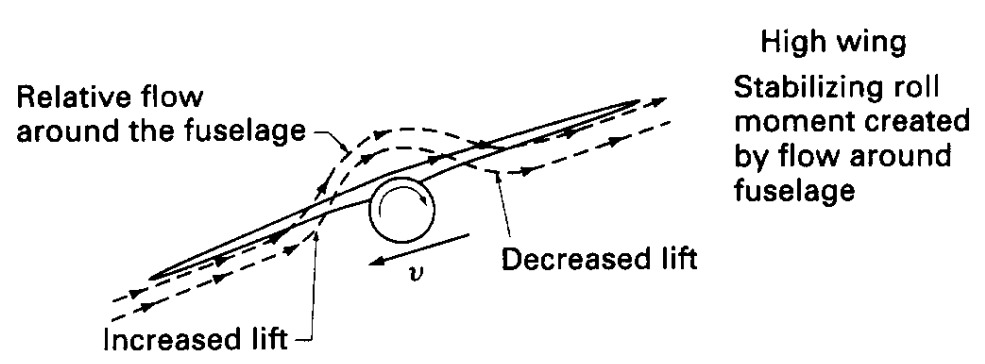
\includegraphics[width=\linewidth]{Codes/Week 6/wing configuration.jpeg}
    \caption{High Wing configuration}
    \label{High Wing configuration}
\end{figure}
\color{red}
\subsection{Wing Design}
\color{black}
The following are the detailed wing parameters that were previously estimated.
\begin{table}[H]
\centering
\begin{tabular}{|l|l|}
\hline
\textbf{Parameters} & \textbf{Values} \\
\hline
Reference Area (S) & 0.7 sq.m \\
Wing Geometry & Rectangular Wing \\
Aspect Ratio (AR) & 7.175 \\
Wingspan (b) & 2.241093483 m \\
Chord (c) & 0.312347524 m \\
\hline
\end{tabular}
\caption{Wing Parameters}
\label{tab:wing_parameters}
\end{table}
\begin{figure}[H]
    \centering
    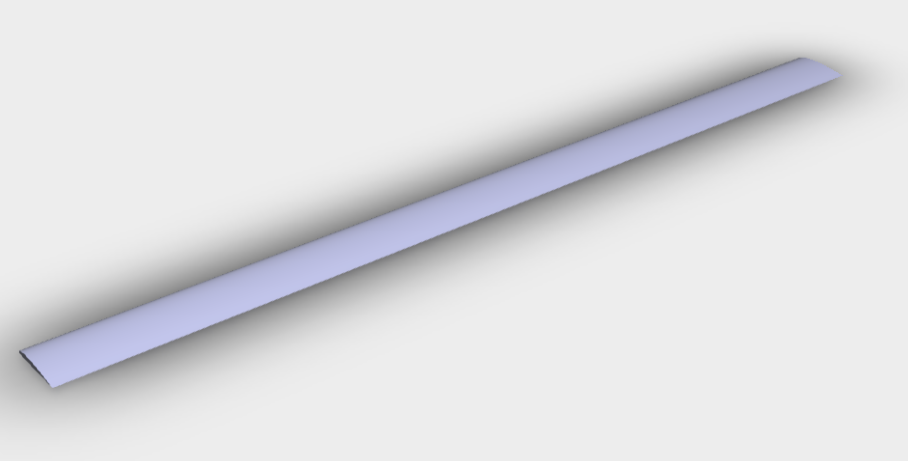
\includegraphics[width=1.0\linewidth]{3d_wing.png}
    \caption{3D MODEL OF RECTANGULAR WING}
    \label{3D MODEL OF RECTANGULAR WING}
    \end{figure}
\color{red}
 \large{\underline{Taper ratio}}
\color{black}
\vspace{5mm}
\\Taper ratio refers to the ratio of the wingtip chord to the wing root chord, providing insight into the shape of the wing planform. A taper ratio of 1 indicates a rectangular wing, where the chord length remains constant from the wing root to the wingtip. This configuration is contrasted with tapered wings, where the chord decreases progressively from the root to the tip.

Rectangular wings offer several advantages over tapered wings. Firstly, they provide more straightforward structural design and analysis due to their uniform geometry, facilitating ease of fabrication and reducing manufacturing complexities. Additionally, rectangular wings typically exhibit more predictable aerodynamic characteristics, especially at low speeds, simplifying flight performance analysis and enhancing overall stability. Moreover, the uniform chord distribution of rectangular wings often results in improved stall behavior and handling characteristics, making them preferable for specific applications, such as UAVs operating in varied flight conditions.

 Given these considerations, the decision to adopt a rectangular wing configuration in which the\textbf{ Taper ratio = 1 }is taken.\\

\color{red}
\large{\underline{Wing Setting Angle $i_w$}}\\
\\ \color{black}
The wing setting angle, denoted as \( i_w \), refers to the Angle at which the wing is positioned relative to the aircraft's fuselage or horizontal reference plane. It is crucial in determining an aircraft's aerodynamic performance and stability characteristics during flight.

A positive wing setting angle typically results in a nose-up attitude, generating more lift but potentially increasing drag. Conversely, a negative setting angle may reduce lift while enhancing aerodynamic efficiency. The optimal setting angle depends on various factors, including aircraft design, mission requirements, and flight conditions.

As the desired lift coefficient has been achieved in our wing design,  we are maintaining the wing setting angle at 0 degrees. This indicates that the wing is positioned parallel to the horizontal reference plane. This configuration also suggests an optimal balance between lift generation and drag minimization, aligning with the desired aerodynamic performance criteria for the aircraft's mission profile.\\
\\ \vspace{10mm}
\color{red}
\large{\underline{Wing Sweep and Geometric Twist}}\\
\color{black}
Wing sweep refers to the Angle at which the wings are inclined backward from the root to the tip. This feature can enhance aerodynamic efficiency by reducing drag at high speeds, improving stability, and delaying the onset of compressibility effects. On the other hand, a geometric twist involves varying the Angle of incidence along the span of the wing, typically with a higher angle of incidence at the wing root and decreasing towards the wingtip. Geometric twist helps to optimize lift distribution and stall characteristics across the wing span.

In our wing design, wing sweep and geometric twist are not utilized due to concerns related to fabrication complexity. Incorporating these features would require intricate structural design and manufacturing processes, potentially increasing production costs and time. Additionally, wing sweep and twist could introduce structural challenges and compromises in aerodynamic performance.

Furthermore, the decision not to employ winglets, which are small wing-like structures often added to the wingtips, is made to further simplify the design and manufacturing process. While winglets can reduce induced drag and improve fuel efficiency, their integration adds complexity to the wing design and may not benefit the intended mission profile significantly.\\
\\ \vspace{5mm}
\color{red}
\large{\underline{Ailerons}}\\
\color{black}
Ailerons are control surfaces typically located on the wing's trailing edge near the wingtips. They control the aircraft's roll motion by deflecting in opposite directions. When one aileron moves upward, the other moves downward, causing the aircraft to roll about its longitudinal axis.

In our wing design, placing the ailerons is crucial for optimizing control effectiveness and aerodynamic performance. Therefore, the ailerons will be positioned at specific locations along the wing. Specifically, they will be located between \textbf{0.5 to 0.96 of the wing's span}, ensuring sufficient leverage for roll control across the entire wing length. Additionally, the ailerons will span from \textbf{0.8 to 1 of the wing's chord}, providing adequate surface area for effective control authority while maintaining aerodynamic efficiency.
\newpage
\textbf{\Huge{Chapter 7}}
\section{\underline{Fuselage Design}}
\color{red}
\subsection{Fuselage Length}
\color{black}
{The fuselage length in a UAV design is a crucial parameter that affects the overall performance and functionality of the aircraft. It is typically estimated based on the maximum takeoff weight (\(W_0\)) of the UAV. One common approach is to use empirical relationships derived from data on similar aircraft.}

{The fuselage length (\(L\)) is often modeled using a power-law relationship with the maximum takeoff weight (\(W_0\)). This relationship can be expressed as:}

\textbf{\[ L = a W_0^c \]}

where:
\begin{itemize}
    \item \(L\) is the fuselage length,
    \item \(W_0\) is the maximum takeoff weight,
    \item \(a\) and \(c\) are parameters obtained through curve fitting.
\end{itemize}
\begin{table}[htbp]
  \centering
  \caption{\textbf{UAV Maximum Takeoff Weight (MTOW) and Fuselage Length}}
  \begin{tabular}{|l|c|c|}
    \hline
    \textbf{UAV} & \textbf{MTOW (N)} & \textbf{Fuselage Length (m)} \\
    \hline
    Wingtraone & 44.145 & 0.66 \\
    Albatross & 98.1 & 0.8 \\
    Azimut 2 & 88.29 & 1.7 \\
    Birdeye 600 & 83.385 & 1.2 \\
    Rafael Skylite BR & 78.48 & 0.91 \\
    Bluebird Boomerang & 93.195 & 0.95 \\
    \hline
  \end{tabular}
\end{table}
\begin{figure}[H]
    \centering
    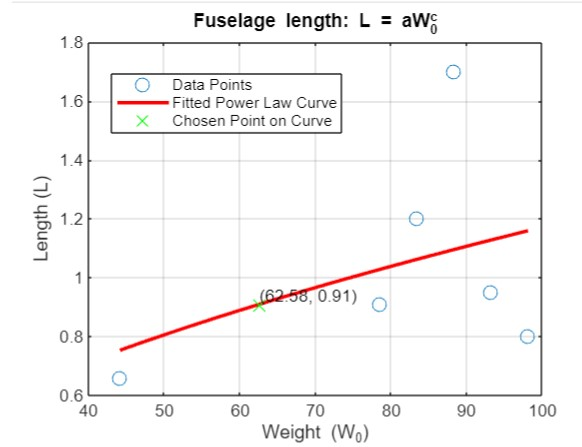
\includegraphics[width=\linewidth]{Codes/Week 6/Fuselage length curve fit.jpg}
    \caption{\textbf{Fuselage length Curve Fit}}
    \label{Fuselage length curve fit}
\end{figure}
\color{red}
\subsection{Curve Fitting and Parameter Estimation}
\color{black}
The parameters \(a\) and \(c\) are typically obtained by fitting the curve to empirical data. Once the best-fit curve is obtained, the values of \(a\) and \(c\) are determined. 

In our case, after conducting curve fitting using MATLAB, we obtained the following parameter values:
\[ a = 0.097577 \]
\[ c = 0.53969 \] 
\newpage
\subsection{\textcolor{red}{Fuselage Length Calculation}}
\color{black}
For a given design weight \(W_0\), the fuselage length can be calculated using the relation obtained from curve fitting. 

For a design weight(\(W_0 = 63.52\) N), the fuselage length (\(L\)) is calculated as follows:

\[
L = 0.3117 \times (63.52)^{0.6156} = 0.91 \, \text{m}
\]

This calculated fuselage length provides valuable insight into the overall dimensions and proportions of the UAV, aiding in the design and optimization process.
\color{red}
\subsection{Fuselage Sizing}
\color{black}
\vspace{10mm}
\section{\underline{Tail Design}}
\color{red}
\subsection{Tail configuration}

{\color{red}\textbf{Conventional Tail (T-tail):}}

{\color{black}
\textbf{\textcolor{red}{Advantages:}}
\begin{itemize}
  \item Provides better pitch control and stability.
  \item Reduces the risk of tail strikes during takeoff and landing.
  \item Simplifies the fuselage design by allowing a clean wing-to-fuselage junction.
\end{itemize}

\textbf{\textcolor{red}{Disadvantages:}}
\begin{itemize}
  \item May experience deep stall phenomenon, where the airflow over the tail is disrupted, leading to loss of control.
  \item More complex control systems may be required to mitigate deep stall risks.
  \item Increased structural complexity and weight due to the need for longer tail structures.
\end{itemize}
}

{\color{red}\textbf{T-tail Configuration:}}

{\color{black}
\textbf{\textcolor{red}{Advantages:}}
\begin{itemize}
  \item Offers improved stability and control, especially at high angles of attack.
  \item Reduces the risk of deep stall compared to conventional tail configurations.
  \item Provides redundancy in case of damage to one tail surface.
\end{itemize}

\textbf{\textcolor{red}{Disadvantages:}}
\begin{itemize}
  \item Increased weight and drag compared to single-tail configurations.
  \item Higher manufacturing and maintenance costs due to the complexity of two tail surfaces.
  \item Can obstruct the airflow over the horizontal stabilizer, reducing efficiency.
\end{itemize}
}

{\color{red}\textbf{H-tail Configuration:}}

{\color{black}
\textbf{\textcolor{red}{Advantages:}}
\begin{itemize}
  \item Offers excellent longitudinal stability and efficient pitch control.
  \item Provides a balance between stability, control, and structural simplicity.
  \item Pilots benefit from good pitch authority.
\end{itemize}

\textbf{\textcolor{red}{Disadvantages:}}
\begin{itemize}
  \item Risk of tail strikes during takeoff or landing.
  \item Potential interference drag due to the presence of vertical tails.
  \item Additional weight and drag compared to some other configurations.
\end{itemize}
}

{\color{red}\textbf{V-tail Configuration:}}

{\color{black}
\textbf{\textcolor{red}{Advantages:}}
\begin{itemize}
  \item Offers reduced drag and weight compared to conventional tail configurations.
  \item Provides efficient control in both pitch and yaw.
  \item Simplifies the aircraft's structure and reduces radar cross-section in military applications.
\end{itemize}

\textbf{\textcolor{red}{Disadvantages:}}
\begin{itemize}
  \item Can experience control coupling issues, especially in certain flight regimes.
  \item Requires more complex control systems to manage control interactions.
  \item May be less effective at high angles of attack compared to other tail configurations.
\end{itemize}


\vfill

\clearpage

\newpage
\textbf{\Huge{Appendix}}
\appendix


\section{References}
\bibliographystyle{plainnat}
%\bibliographystyle{IEEEtran}
\bibliography{References}

\vspace{10 pt}

The GitHub account having all the codes can be accessed as: - 

\href{https://github.com/abhijeetmangela/Group_7_design.git}{\text{https://github.com/abhijeetmangela/Group\textunderscore 7\textunderscore design.git}}

\newpage

\section{Changes}

\subsection{Week 2}
\begin{enumerate}
    \item The Data collection part was completely changed.
    \item The general design of the pdf was changed.
    \item More data was added along with a table for better comparison.
    \item Battery performance was estimated.
    \item Weight was estimated.
    \item References were added.
    \item The Mission profile was updated.
    \item Details on mission profile were added.
\end{enumerate}

\subsection{Week 3}
\begin{enumerate}
    \item The Weight estimation was redone
    \item Power was estimated for different phases 
\end{enumerate}

\subsection{Week 4}
\begin{enumerate}
    \item Power calculations were recalculated.
    \item Battery was selected.
    \item Motor and propeller were selected.
    \item Wing loading was done
\end{enumerate}

\newpage


\section{Contributions}

\subsection{Week 2}

\subsubsection{Abhijeet Mangela AE21B040}
Wrote full Latek report, Drew the mission profile with Inkscape and Autocad, Empty weight Fraction estimation, and Final weight estimation with Senthil

\subsubsection{Navin Yadav AE23M803}

Data Collection; Literature Survey

\subsubsection{Balamurugan S AE23M009}

Data Collection; Literature Survey

\subsubsection{Samarth R Krishna AE23M032}

Data Collection; Literature Survey

\subsubsection{Senthil B AE23M035}

Detailed Mission Profile; Preliminary Weight Estimation (only iteration); Battery weight estimation.

\subsubsection{Rajendran Anandhu Nair AE23M027}

Data Collection; Literature Survey




\subsection{Week 3}


\subsubsection{Abhijeet Mangela AE21B040}
Changed the Mission Profile in Latex, Converted references to BibTeX, Did some cleanup of the document, did the Preliminary weight estimate, which was wrong last week, Power estimation for cruise and climb, and Linked all files internally in Github for easy connectivity.

\subsubsection{Navin Yadav AE23M803}
The analytical calculation and added these calculations to the latex 

\subsubsection{Balamurugan S AE23M009}
Data Collection; Literature Survey; Max L/D vs Sqrt(Wetted AR) Calculations and Plotting.


\subsubsection{Samarth R Krishna AE23M032}
The analytical calculation (Drag Polar calculation, L/D max estimation, calculation of Thrust and Power required at different phases) and added these calculations to latex.


\subsubsection{Senthil B AE23M035}
Data Collection; Image Processing using ImageJ; Max L/D vs Sqrt(Wetted AR) Calculations and Plotting.


\subsubsection{Rajendran Anandhu Nair AE23M027}
Data Collection; Image Processing using Fusion 360; Report writing for Reference and Wetted areas, Aspect ratios, Coefficient of lift, and Maximum lift-to-drag ratio. 

\subsection{Week 4}


\subsubsection{Abhijeet Mangela AE21B040}
Did Wing loading for stall criteria, the effect of flaps, as well as all $\frac{W}{S}$ calculations for Stall, Takeoff, Landing, Cruise, and loiter and wrote \LaTeX for it.

\subsubsection{Navin Yadav AE23M803}
The analytical calculation and added these calculations to the latex 

\subsubsection{Balamurugan S AE23M009}


\subsubsection{Samarth R Krishna AE23M032}
The analytical calculation (Iterations and calculation of Power required at different phases) added these calculations to latex.


\subsubsection{Senthil B AE23M035}
We calculated power loading for cruise climb descent, loiter, and stall conditions. We also calculated and approximated design parameters like wing reference area.

\subsubsection{Rajendran Anandhu Nair AE23M027}
Calculated battery capacity required for each mission segment based on their power requirements. A selected battery, motor, and propeller are required for the UAV. Wrote the power loading, battery capacity, and powerplant selection parts in LATEX. 


\newpage

\section{Current estimates}
\begin{itemize}
    \item Range- 20 Km
    \item Endurance- 30 min
    \item Payload- 1.4 kg
    \item Total weight- 6.5 Kg
\end{itemize}

\end{document}
